%-----------------------------------------------------------------------------%
%                                                                             %
%    K A P I T E L   5                                                        %
%                                                                             %
%-----------------------------------------------------------------------------%

\chapter{Highly-Dynamic Movements}\label{c5}
This chapter presents an analysis of the proposed motion planning approach for highly-dynamic movements of the full-size humanoid RH5. To begin with, the central building blocks of the optimization problem are again briefly addressed. Then the simulation results for jumping tasks of increasing complexity are presented. Finally, an analysis of the maximal system performance based on the allowed joint and torque limits is presented.  


\section{Formulation of the Optimization Problem}\label{sec:HighlyFormulation}
This section concisely summarizes the constraints of the \gls{OC} problem used to generate highly-dynamic movements as demonstrated in the following up section. 

The vertical jump formulation follows an optimization problem of the form described in \cref{eqn:optimizationProblem}. For performing multiple forward jumps over obstacles instead, we successively solve $P$ individual optimization problems of range $N$ for each jump. To this end, we formulate a multi-phase \gls{OC} problem as follows: 
\begin{equation}\label{eqn:optimizationProblemSequence}
\myM{X}^*,\myM{U}^*= 
\arg\min_{\mathbf{X},\mathbf{U}} \sum_{p=0}^{P}
\sum_{k=0}^{N-1} \int_{t_k}^{t_k+\Delta t} l_p(\mathbf{x},\mathbf{u})dt. 
\end{equation} 

We constrain the optimization based on the building blocks introduced in \cref{sec:BipedFormulation}. Precisely, we define a foot tracking cost $\Phi_1$ based on piecewise-linear functions to incorporate the basic jumping height and length. We apply the contact stability constrained \gls{DDP} (\cref{c3}) with dedicated cost functions for \gls{CoP} ($\Phi_3$) and friction cone ($\Phi_4$). Physical compliance is ensured via the torque bounds of the solver and joint limits costs $\Phi_5$. We use a \gls{CoM} tracking cost $\Phi_2$ only for the final stabilization of the motion. Additionally, torque minimization ($\Phi_6$) and posture regularization ($\Phi_7$) are optimized.

Biomechanical studies have shown that the effect of arm swinging is elementary for the performance in human jumping \cite{harman1990effects}. To this end, we also include the arms in the optimization for our jumping tasks. 
In order to account for the dynamic nature of the movements, it turned out to be useful to reduce the integration step size. We found a higher feasibility of the jumping tasks with an integration step size of 10 ms compared to 30 ms for the bipedal walking gaits (see \cref{sec:BipedSimulation}). Since we do not use a contact planner along with this work, the contact timings had to be chosen to approximately match the physic of flight phases. 
Highly dynamic movements are subject to higher impulse forces than is the case with walking movements. As described in \ref{sec:TheoryDDP}, \gls{DDP} relies on integration of the system dynamics in each step to obtain the states. The higher impulse forces then in turn cause numerical drifts of higher order in the contact constraints. This effect is visible as drifting of the support feet after touchdown. Through an extensive grid search, we found a set of valid Baumgarte gains that reduce these numerical drifts for highly-dynamic movements.

\section{Simulation Results for Increasing Task Complexity}\label{sec:HighlySimulation}
This section presents the simulation results for three case studies of highly-dynamic movements obtained by solving an optimization problem based on the description in the previous section. First, we study the task of vertically jumping upwards, then we investigate forward jumping and finally we explore a challenging sequence of multiple forward jumps over obstacles.

\subsection{A Simple Vertical Jump}
The analysis of a simple vertical jump is a good example to understand the underlying challenges highly-dynamic movements bring along in the context of numerical optimization.

\begin{table}[t]
\centering
\caption{Vertical jump characteristics and applied optimization constraints.}
\begin{tabular}{|ll|ll|}
\hline
\multicolumn{2}{|l|}{\textbf{Jump Characteristics}} & \multicolumn{2}{l|}{\textbf{Optimization Constraints}} \\ \hline
Jump height:& 10 cm 	& Tasks: 			& Foot ($\Phi_1$) \\ \hline
Total time:& 0.9 s 		& Stability:    & \gls{CoP} ($\Phi_3$), Friction Cone ($\Phi_4$)\\ \hline
Step size:& 0.01 s 	& Limits: 			& Torque ($\Phi_6$)\\ \hline
& 					& Regularization: 	& Posture ($\Phi_7$), Torque ($\Phi_8$)\\ \hline
\end{tabular}
\label{tab:jumpVertical}
\end{table}

The vertical jumping task (see \cref{tab:jumpVertical}) consists of five phases as depicted in \cref{fig:jumpVertical_Snaps}. From the initial position (a), a descending into the jump (b) takes place. Then, an upward motions accelerates the base until the take off (c). The symmetrical flight phase (d) is ended with a touch down (e) followed by a pose recovery (f). 

\begin{figure}[h!]
\begin{subfigure}{.16\textwidth}
	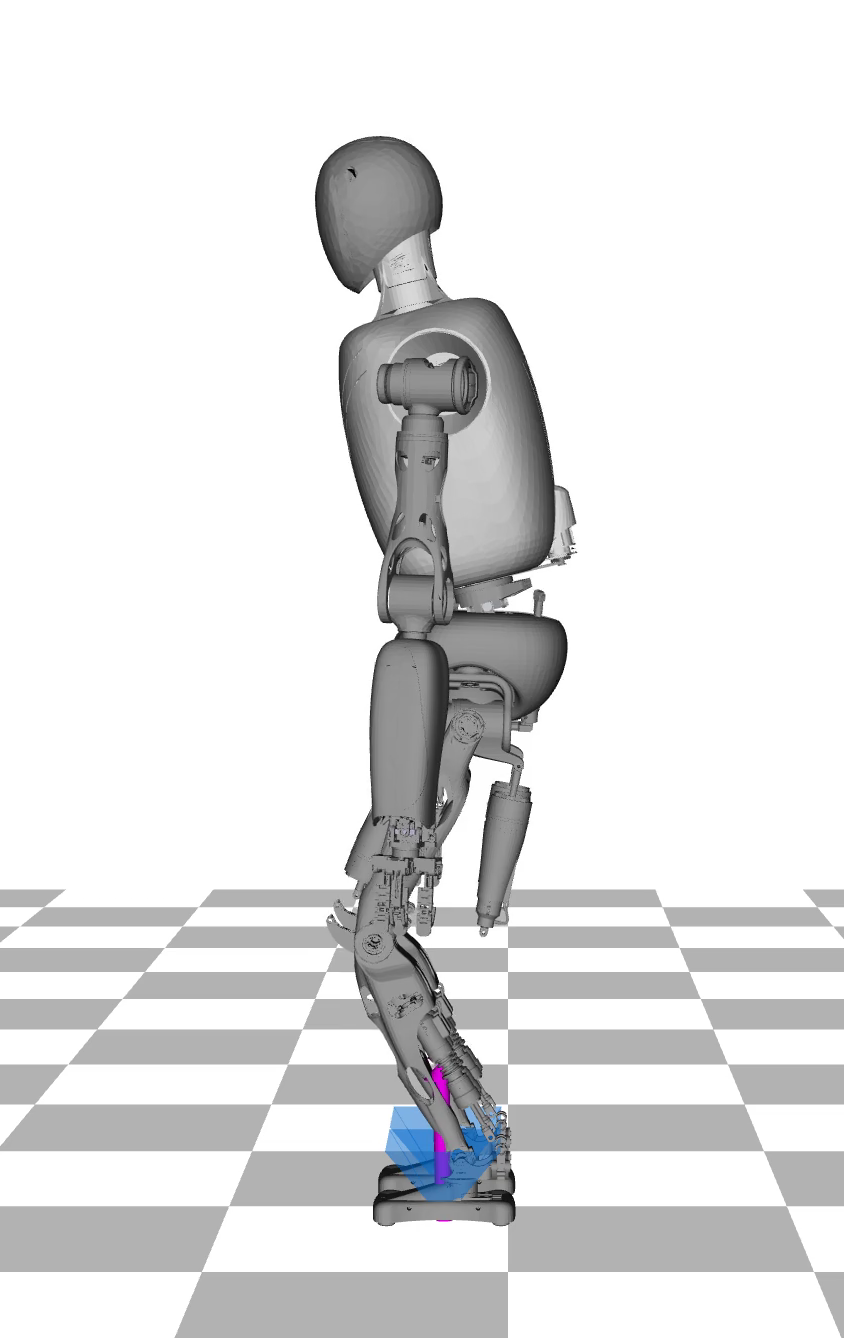
\includegraphics[width=1\linewidth]{fig/jumpVertical/snaps/1x}
	\caption{}
	\end{subfigure}%
\begin{subfigure}{.16\textwidth}
	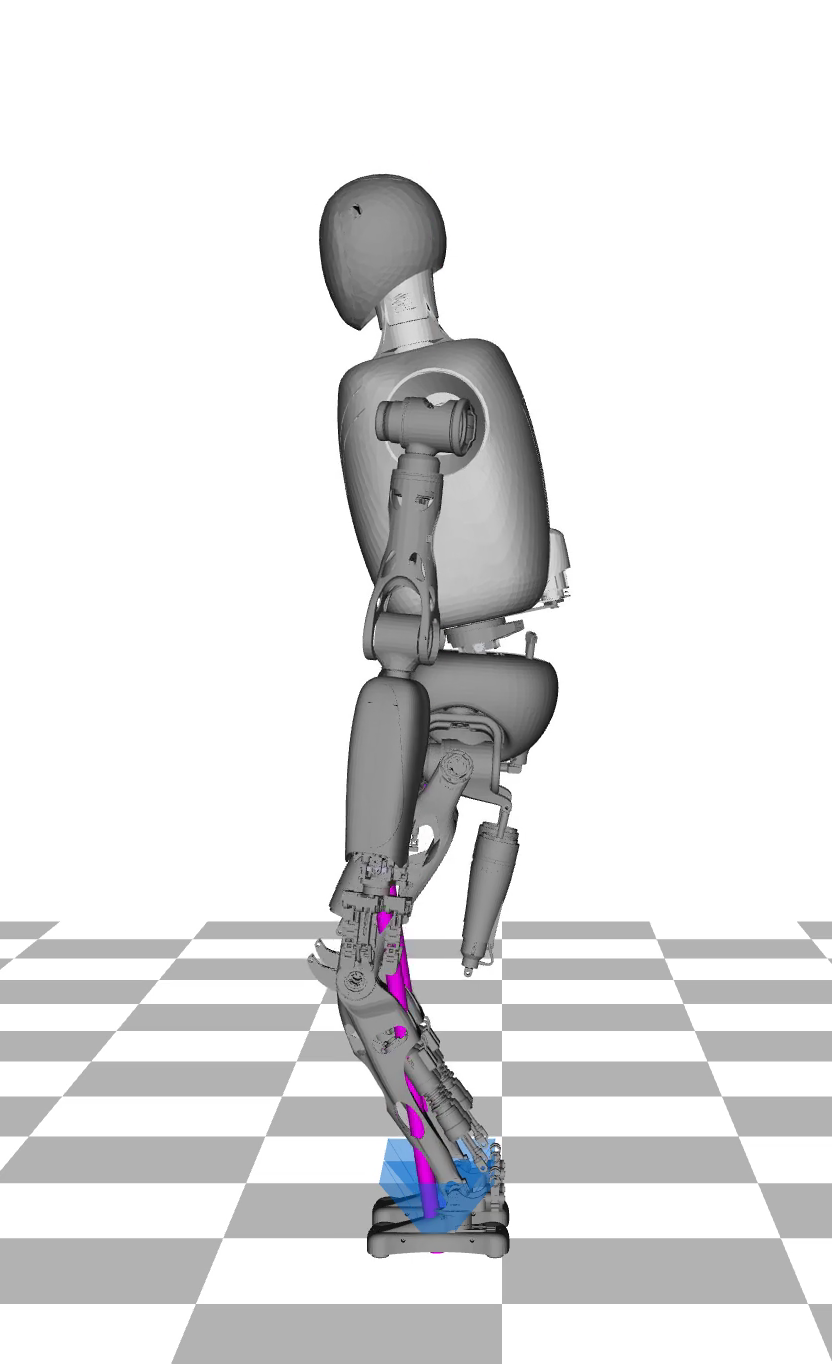
\includegraphics[width=1\linewidth]{fig/jumpVertical/snaps/2x}
	\caption{}
\end{subfigure}%
\begin{subfigure}{.16\textwidth}
	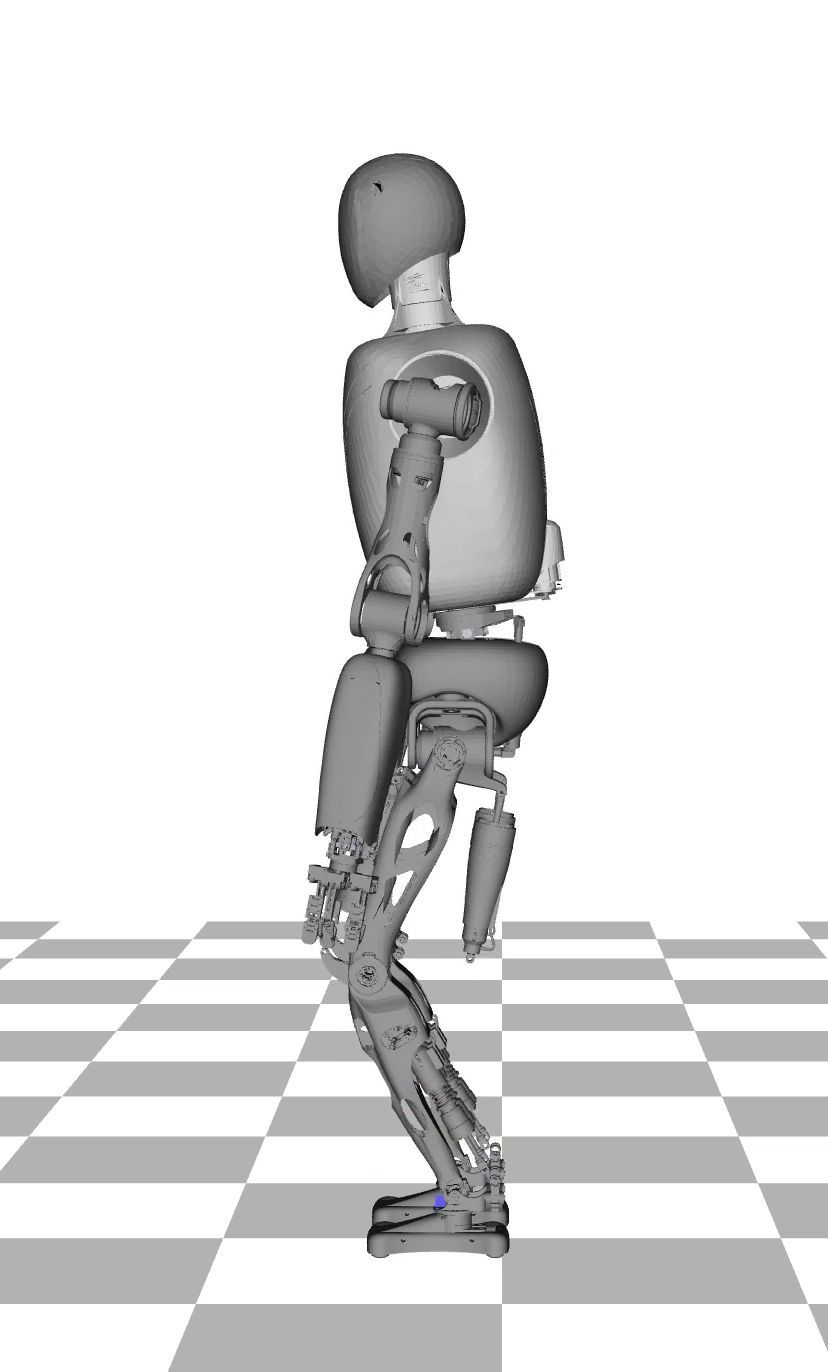
\includegraphics[width=1\linewidth]{fig/jumpVertical/snaps/3x}
	\caption{}
	\end{subfigure}%
\begin{subfigure}{.16\textwidth}
	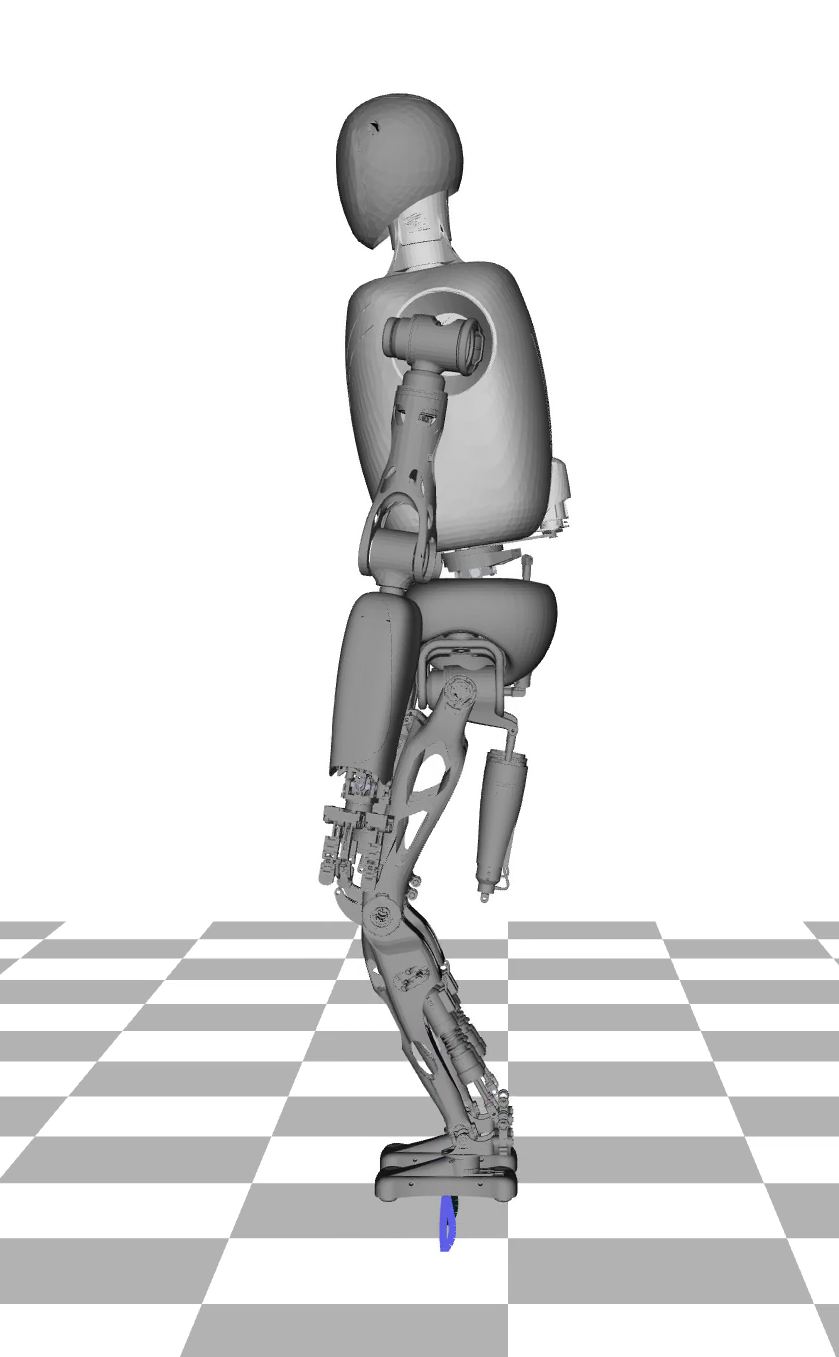
\includegraphics[width=1\linewidth]{fig/jumpVertical/snaps/4x}
	\caption{}
\end{subfigure}%
\begin{subfigure}{.16\textwidth}
	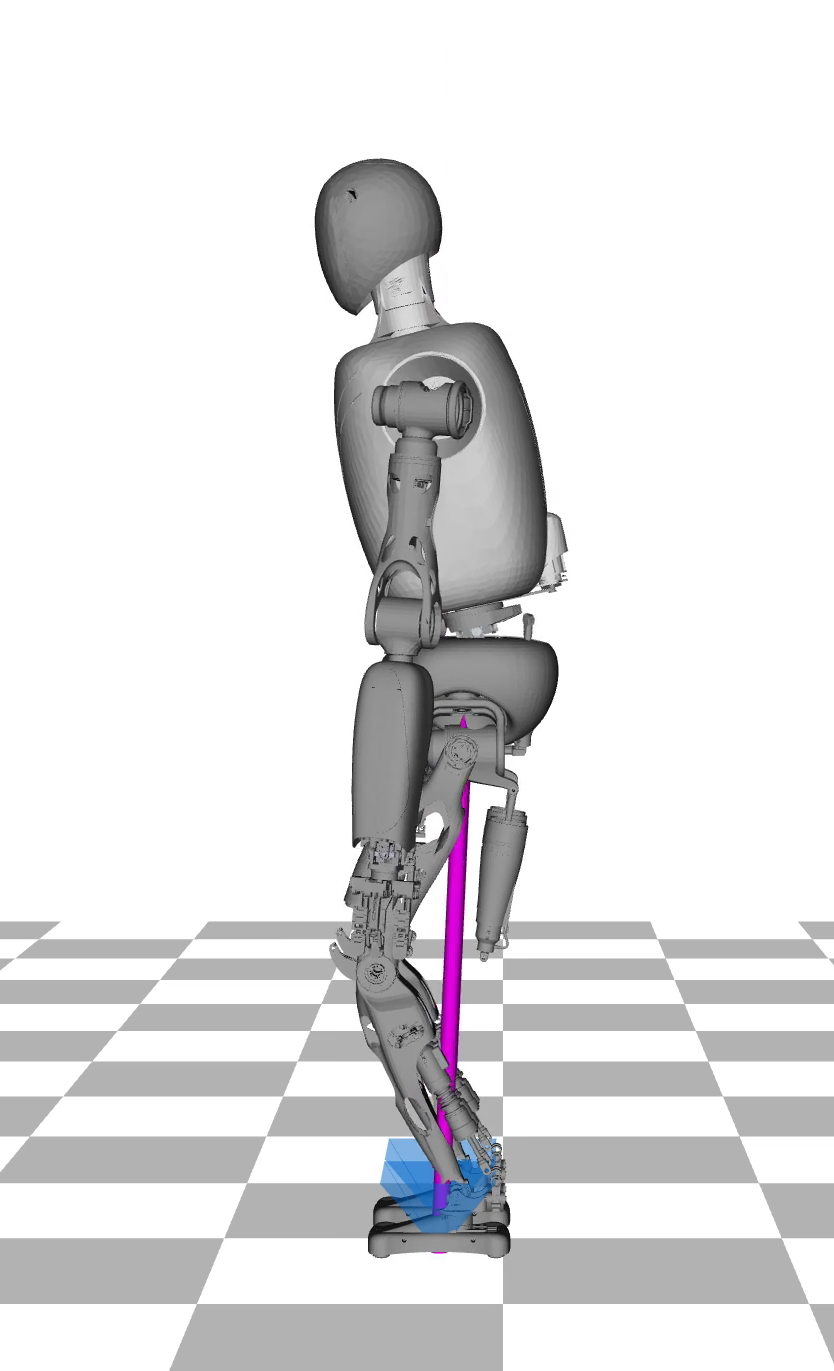
\includegraphics[width=1\linewidth]{fig/jumpVertical/snaps/5x}
	\caption{}
	\end{subfigure}%
\begin{subfigure}{.16\textwidth}
	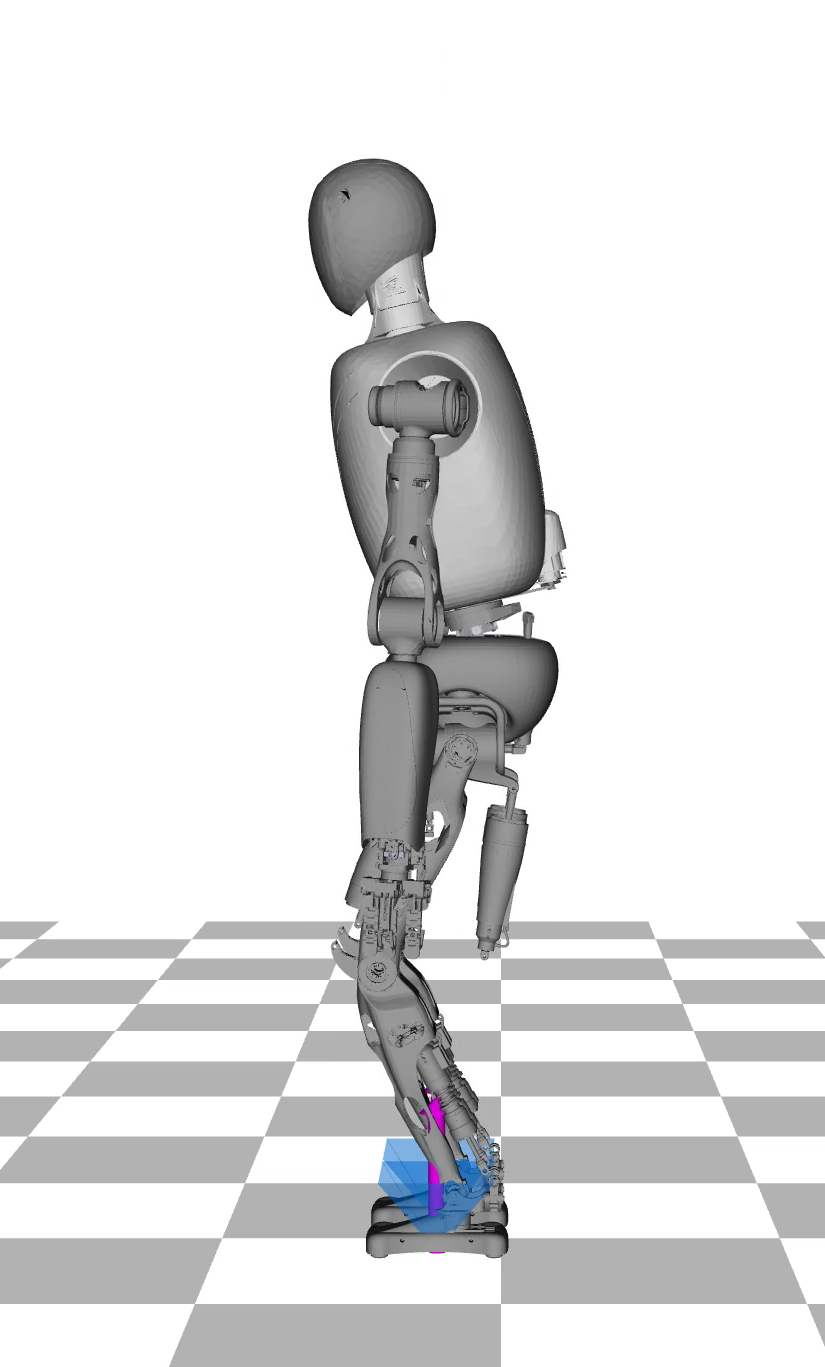
\includegraphics[width=1\linewidth]{fig/jumpVertical/snaps/6x}
	\caption{}
\end{subfigure}%
\caption{A simple vertical jump.}
\label{fig:jumpVertical_Snaps}
\end{figure} 

\cref{fig:jumpVertical_JointState} provides insights in the dynamic nature of the motion. As can be seen, the joint positions stay within reasonable ranges. However, velocity peaks at the take off exceed the maximum joint velocities of the body pitch and knee joints by a factor of two and four, respectively. This effect is plausible, since both the knee deflection as well as the torso swing are essential for a jump. Consequently, the short time horizon of the jump requires high peak velocities in these task-relevant joints. 

\begin{figure}[h!]
\centering	
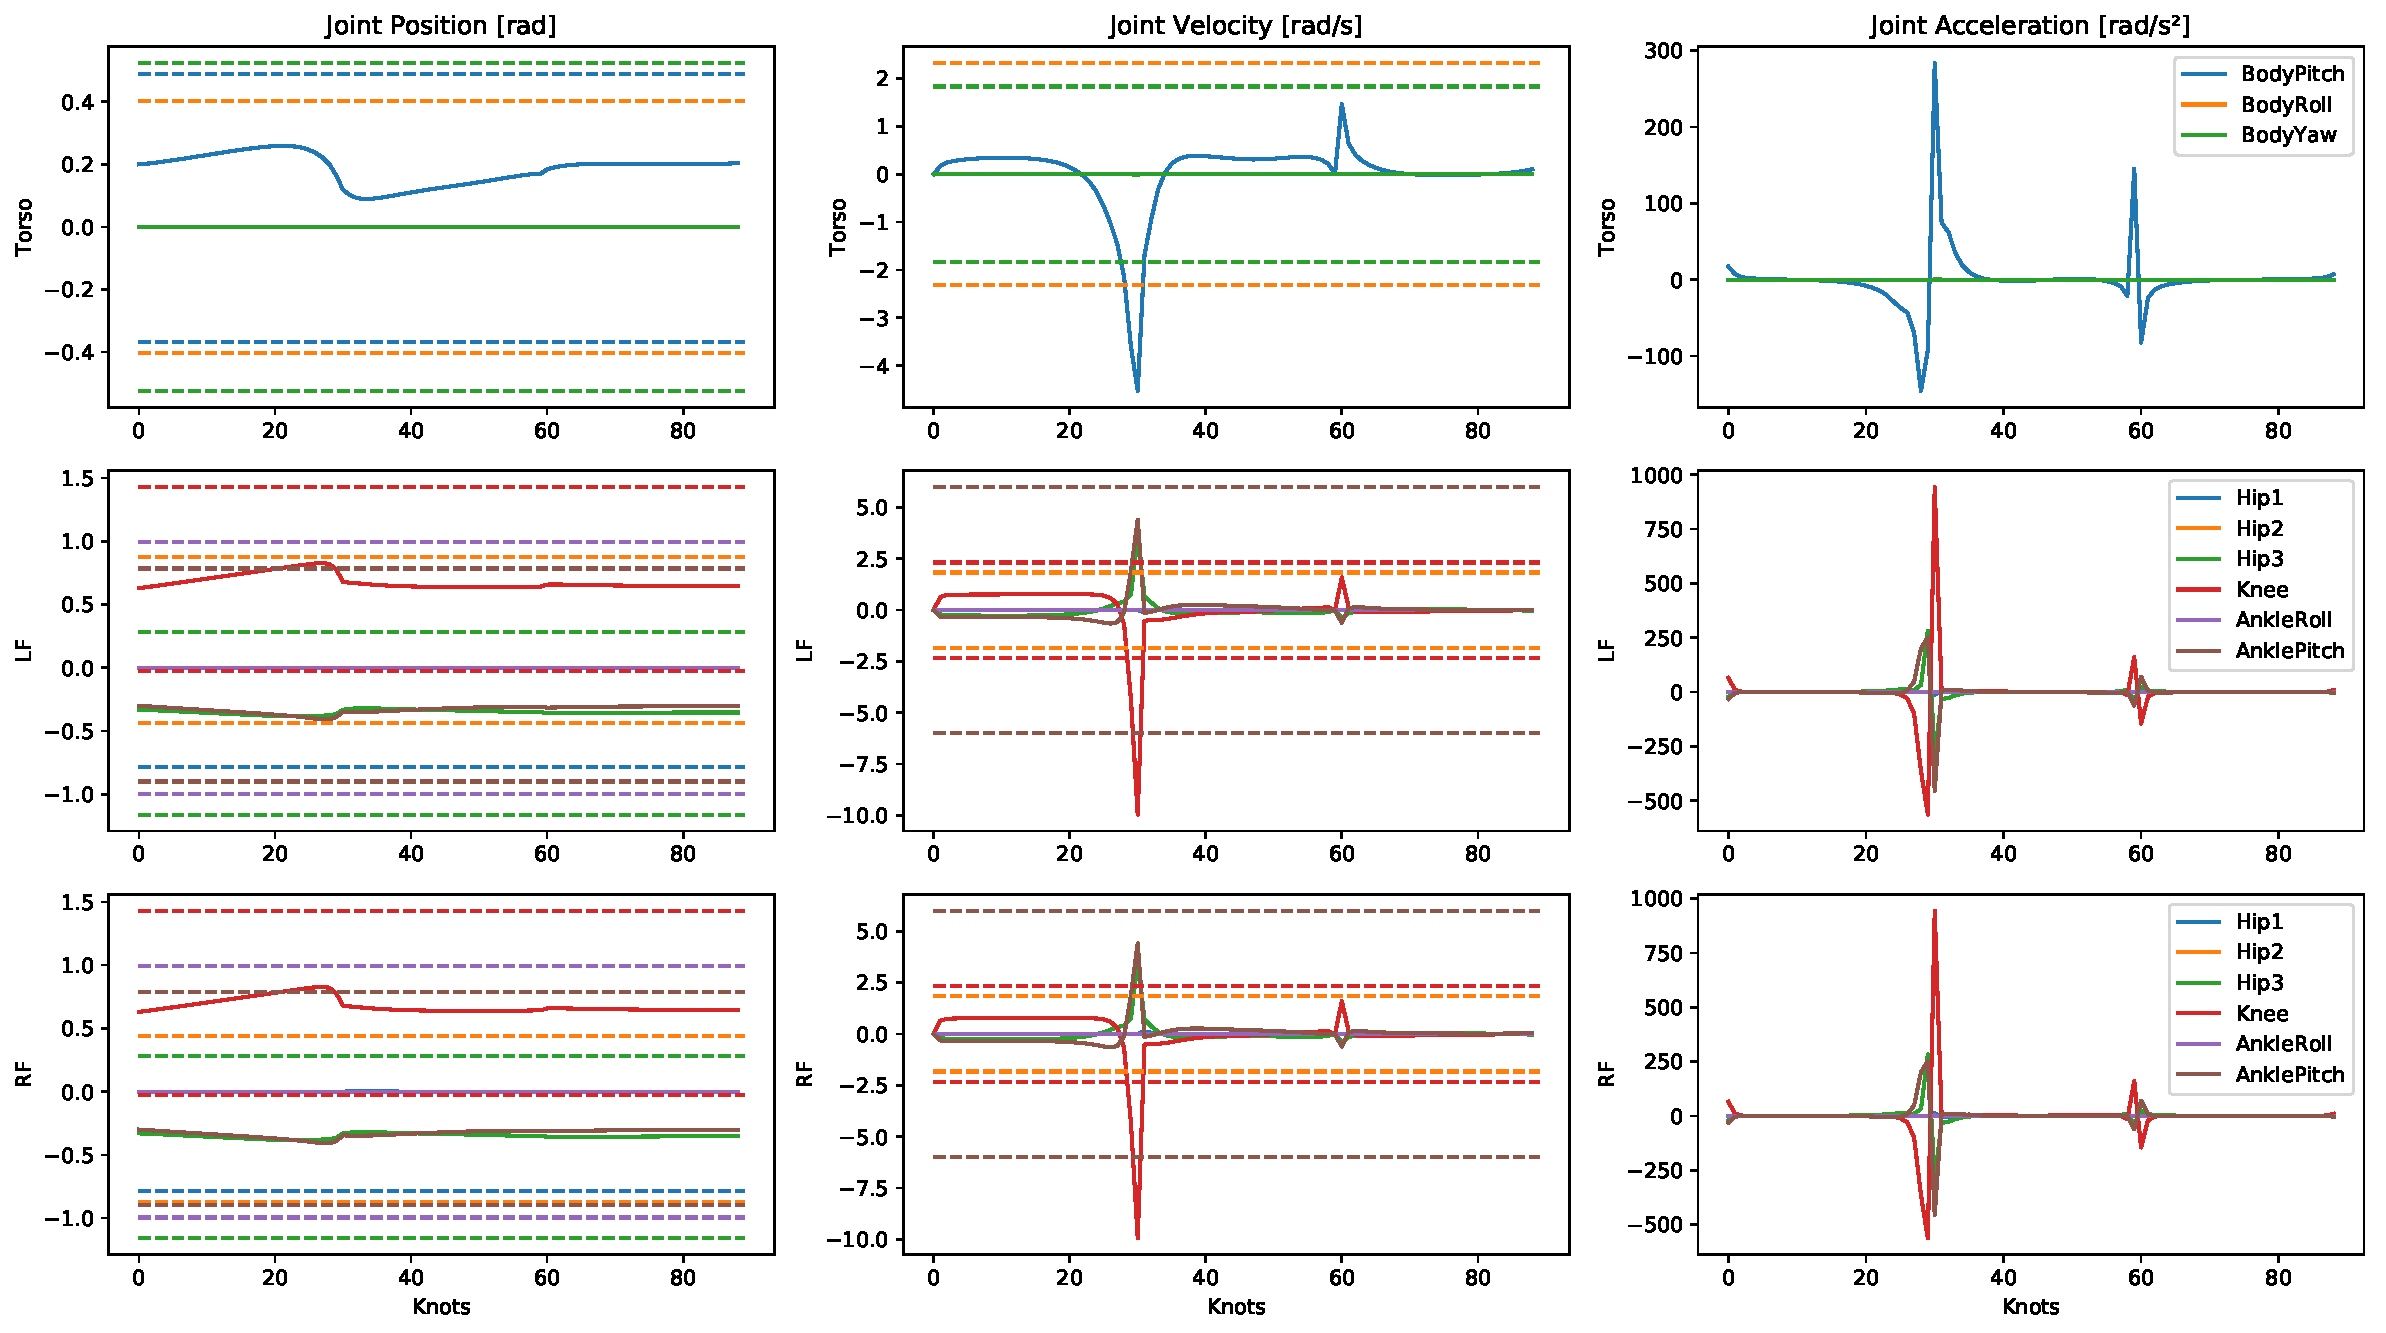
\includegraphics[width=1\textwidth]{fig/jumpVertical/JointState}
\caption{Vertical jump solution of the joint states with according joint limits visualized as dashed lines. The maximum velocities of the body pitch and knee joints turn out to be insufficient for the highly-dynamic take off.}
\label{fig:jumpVertical_JointState}
\end{figure} 

A similar observation applies to the joint torques as shown in \cref{fig:jumpVertical_JointTorques}. Although the solver prevents the body pitch and knee torques to exceed the limits in this case, it becomes evident that maximum torques for these joints are necessary over longer time horizons. Such continuous loads should be avoided as far as possible in order to guarantee the durability of the robotic system.

\begin{figure}[h!]
\centering	
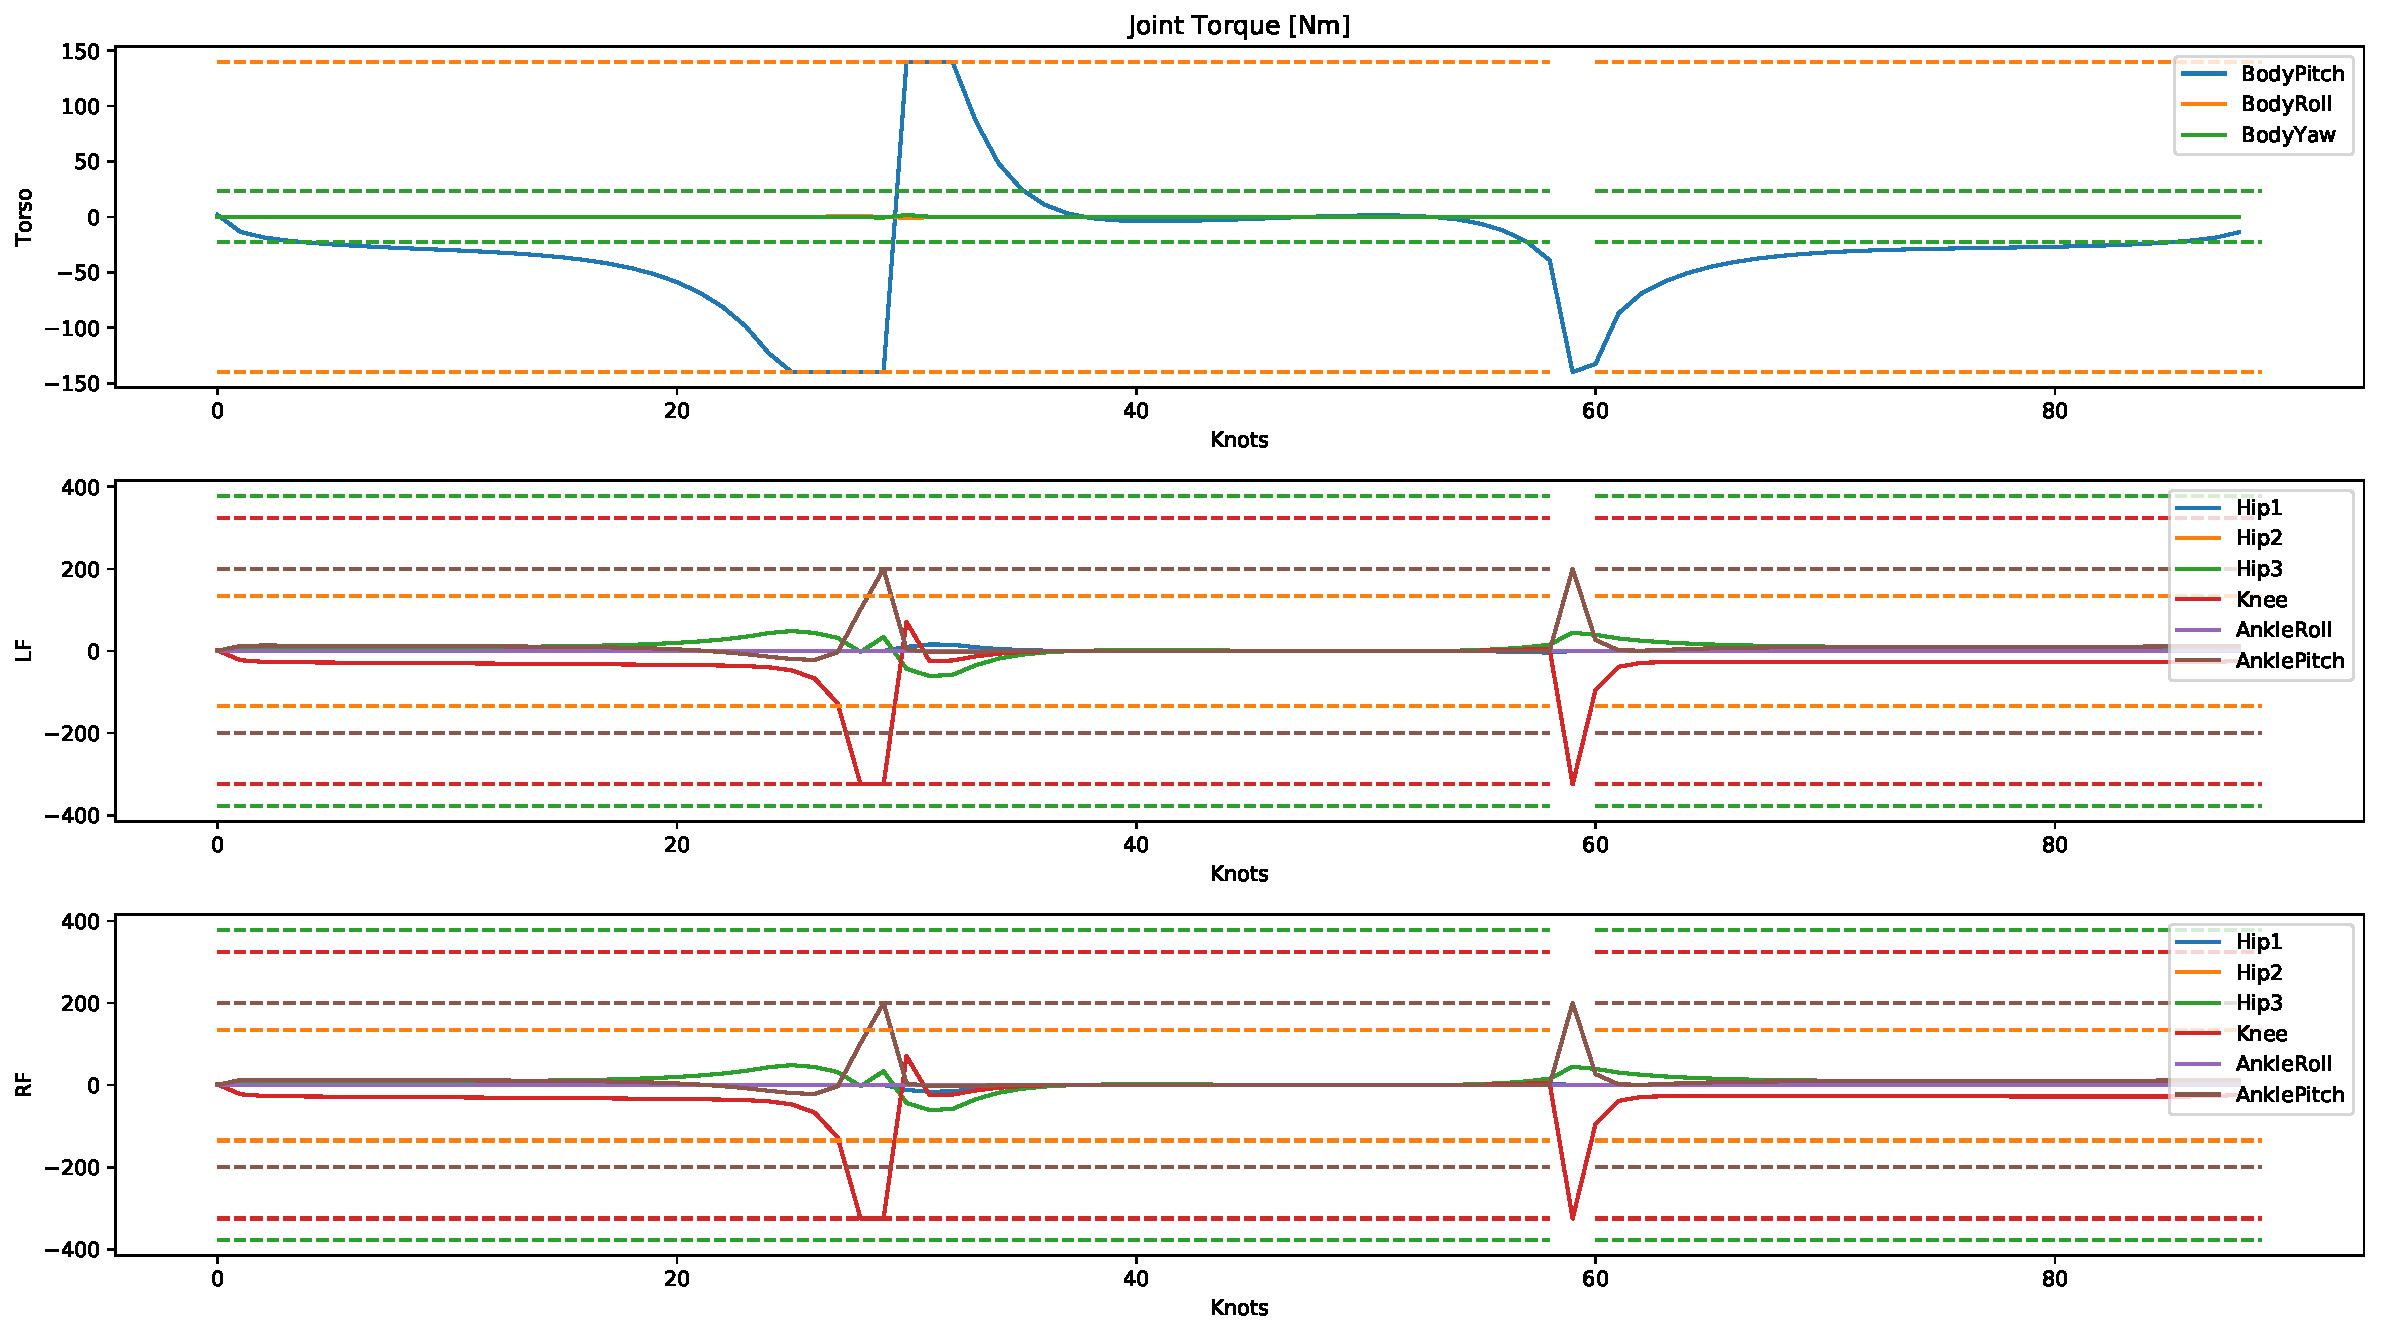
\includegraphics[width=1\textwidth]{fig/jumpVertical/JointTorques}
\caption{Vertical jump solution of the joint torques with according motor limits visualized as dashed lines. The solver prevents the body pitch and knee torques to exceed the limits, but still maximum torques are required for these joints over longer time horizons.}
\label{fig:jumpVertical_JointTorques}
\end{figure} 

\subsection{A Simple Forward Jump}
Focus of investigation is a more dynamic forward jump to study the effect of increasing task complexity on the contact forces and stability.

\cref{tab:jumpForward} summarizes the characteristics and optimization constraints. The forward jumping problem consists of the same five locomotion phases as the vertical jump described previously (see \cref{fig:jumpForward_Snaps}). 
We can draw similar conclusions regarding the physical compliance of the system, namely appropriate joint position ranges and torque limits, but insufficient maximal velocities for the body pitch and knee joints. 

\begin{table}[t]
\centering
\caption{Forward jump characteristics and applied optimization constraints.}
\begin{tabular}{|ll|ll|}
\hline
\multicolumn{2}{|l|}{\textbf{Jump Characteristics}} & \multicolumn{2}{l|}{\textbf{Optimization Constraints}} \\ \hline
Jump length:& 30 cm 	& Tasks: 			& Foot ($\Phi_1$) \\ \hline
Jump height:& 10 cm 	& Stability: 		& \gls{CoP} ($\Phi_3$), Friction Cone ($\Phi_4$)\\ \hline
Total time:& 0.9 s  	& Limits: 			& Torque ($\Phi_6$)\\ \hline
Step size:& 0.01 s   & Regularization: 	& Posture ($\Phi_7$), Torque ($\Phi_8$)\\ \hline
\end{tabular}
\label{tab:jumpForward}
\end{table}

\begin{figure}[h!]
\begin{subfigure}{.16\textwidth}
	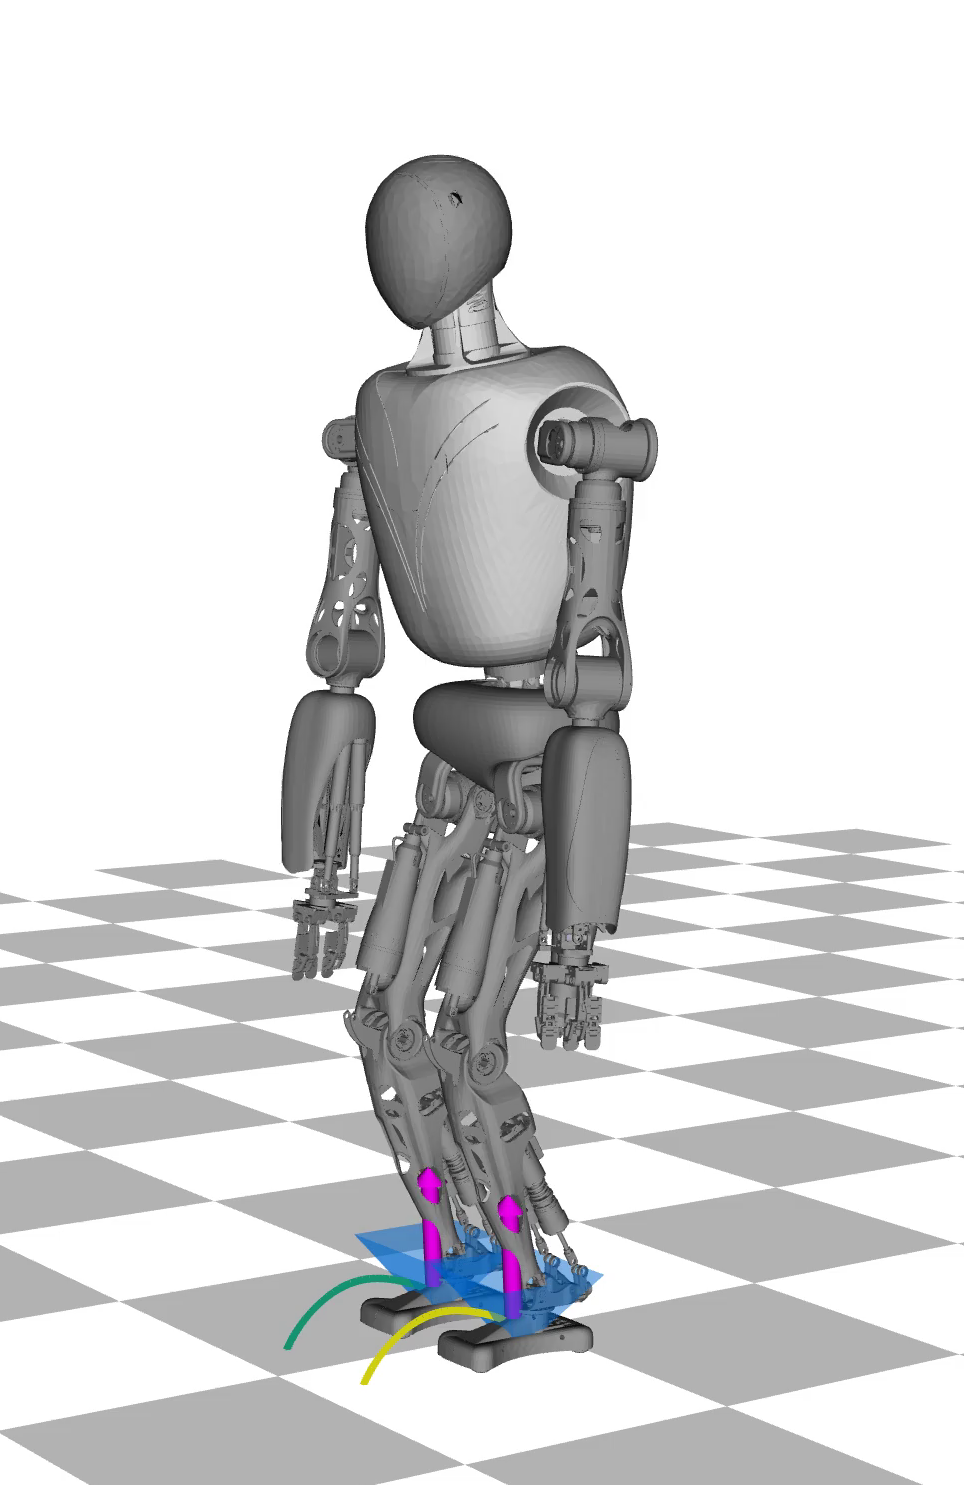
\includegraphics[width=1\linewidth]{fig/jumpForward/snaps/1x}
	\caption{}
	\end{subfigure}%
\begin{subfigure}{.16\textwidth}
	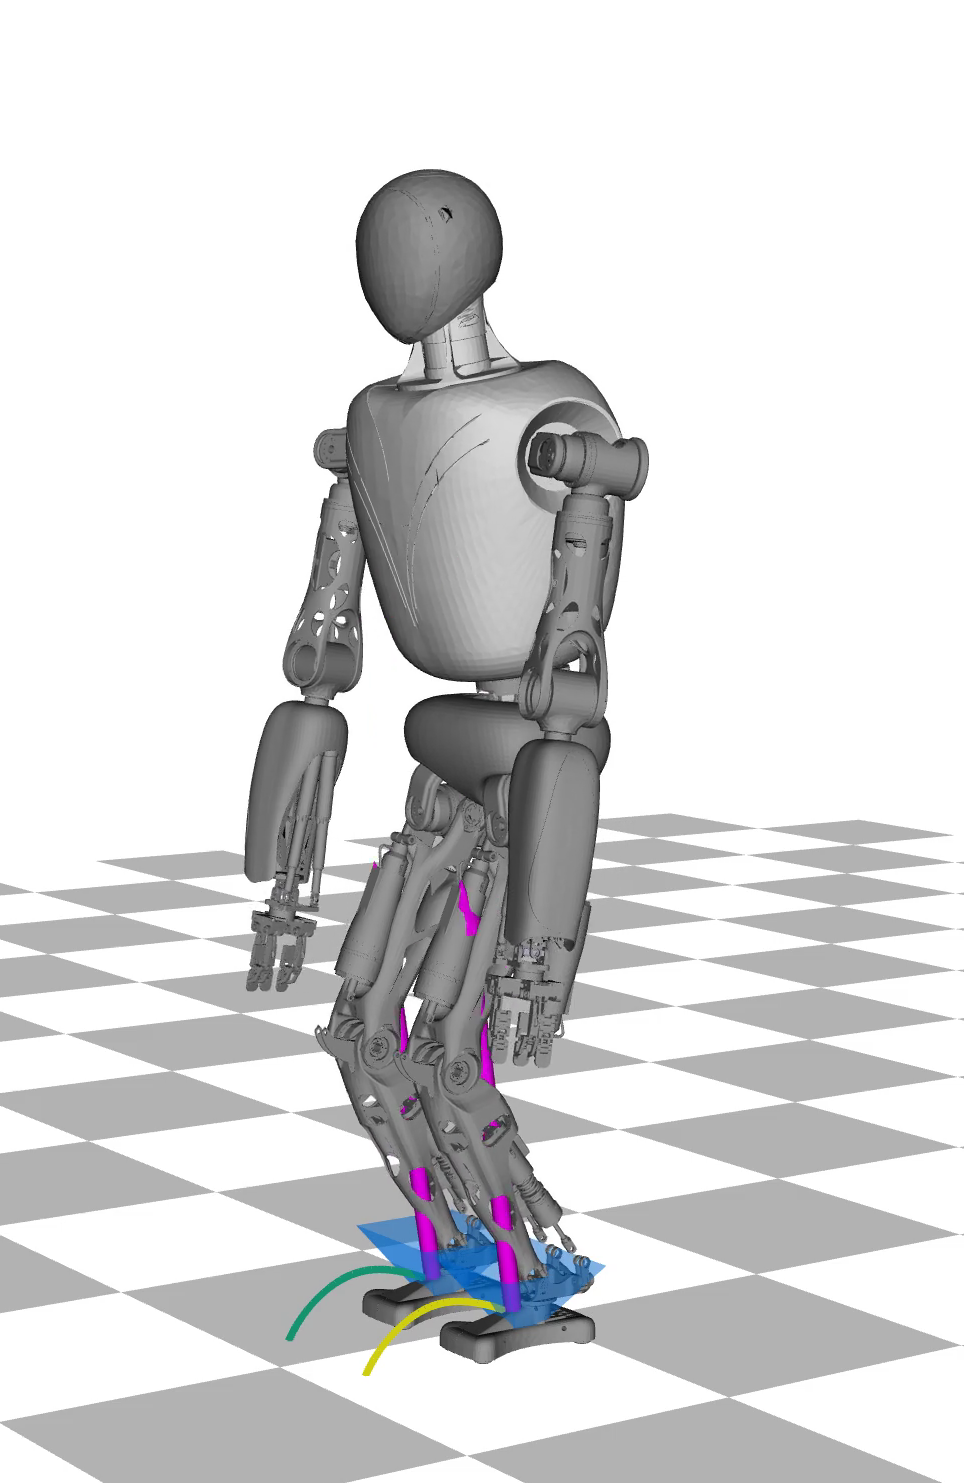
\includegraphics[width=1\linewidth]{fig/jumpForward/snaps/2x}
	\caption{}
\end{subfigure}%
\begin{subfigure}{.16\textwidth}
	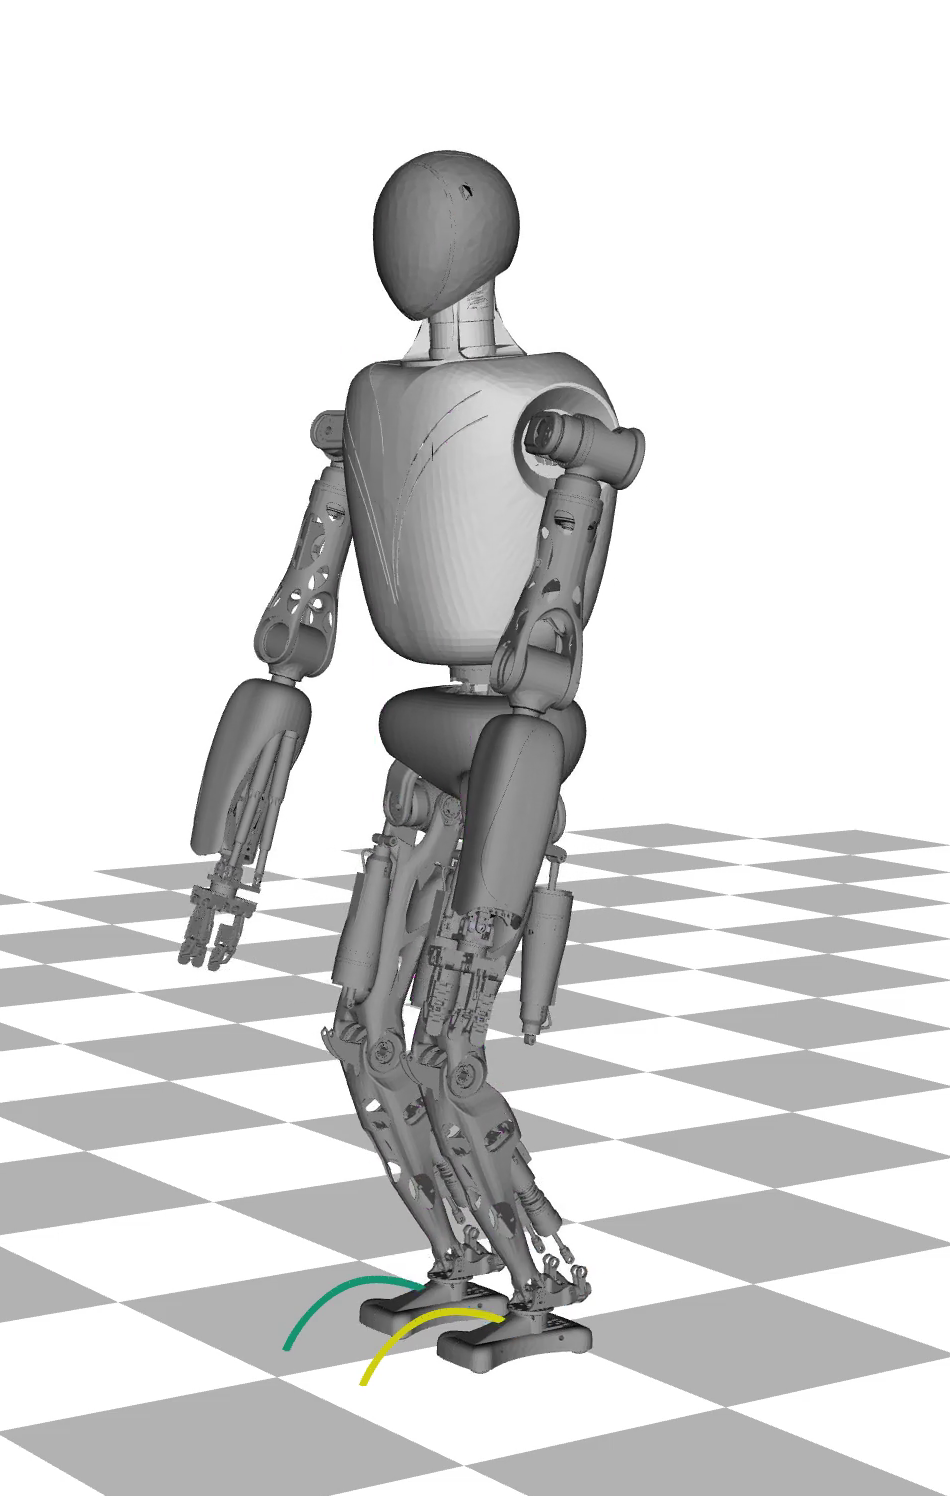
\includegraphics[width=1\linewidth]{fig/jumpForward/snaps/3x}
	\caption{}
	\end{subfigure}%
\begin{subfigure}{.16\textwidth}
	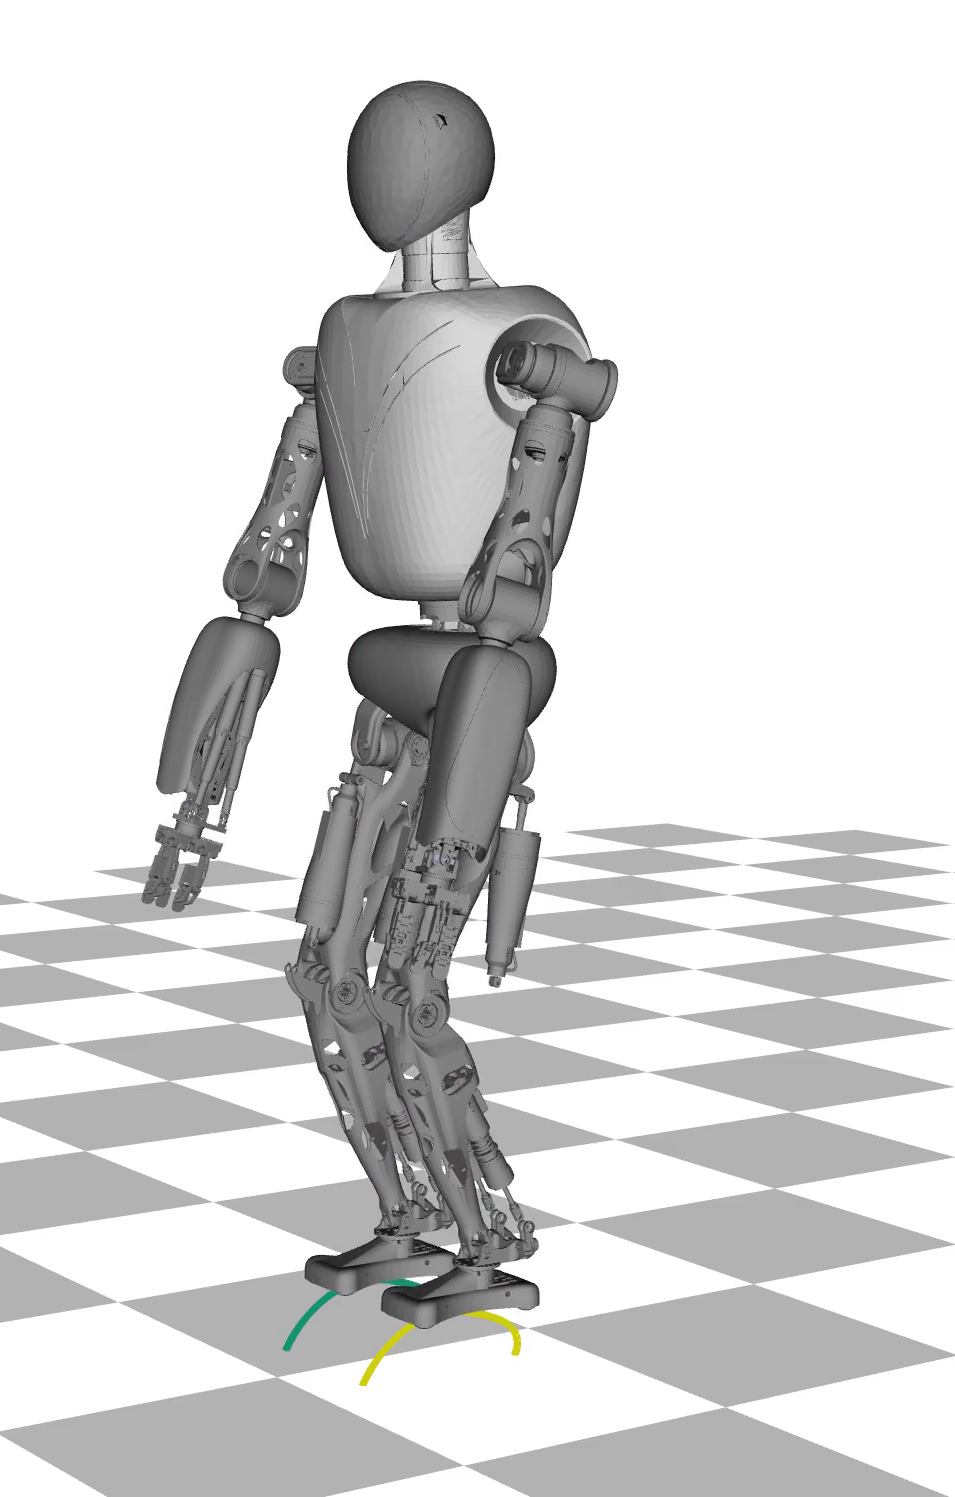
\includegraphics[width=1\linewidth]{fig/jumpForward/snaps/4x}
	\caption{}
\end{subfigure}%
\begin{subfigure}{.16\textwidth}
	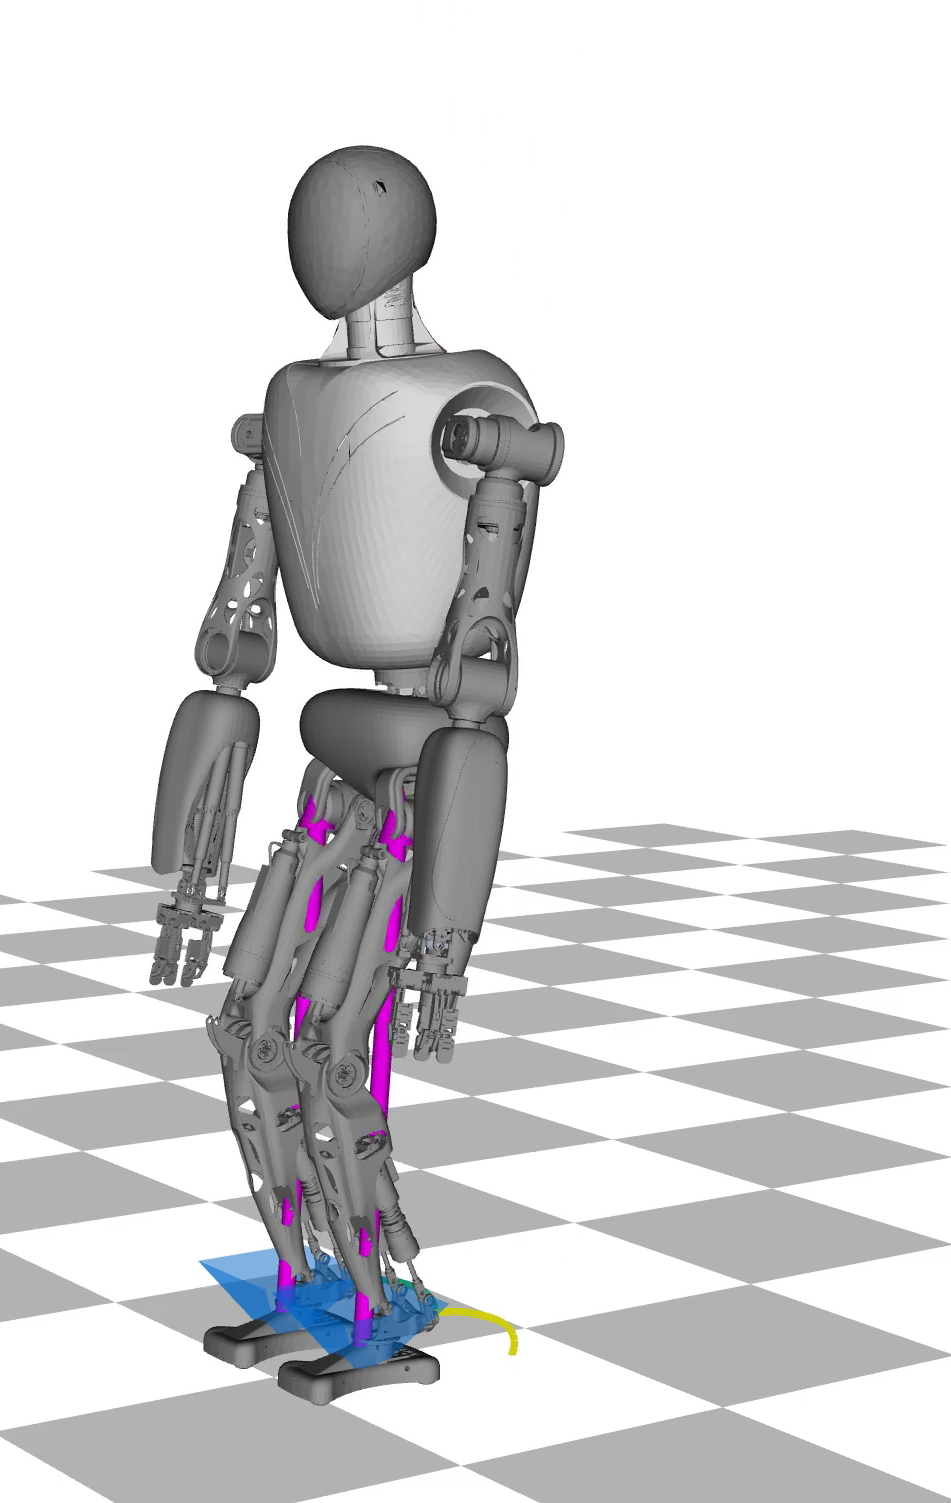
\includegraphics[width=1\linewidth]{fig/jumpForward/snaps/5x}
	\caption{}
	\end{subfigure}%
\begin{subfigure}{.16\textwidth}
	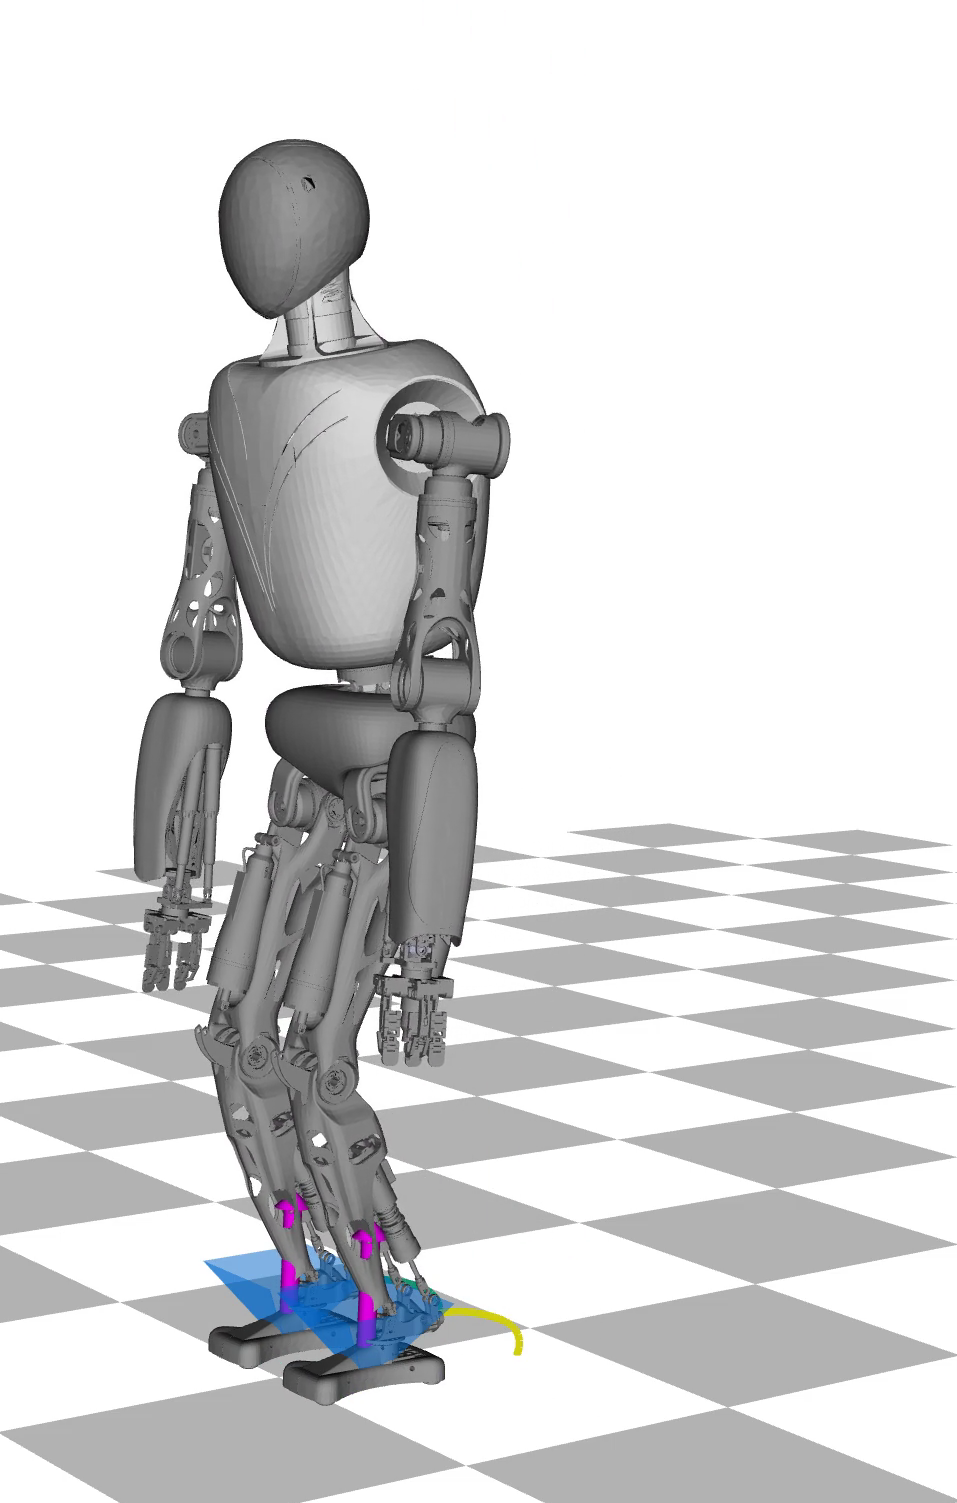
\includegraphics[width=1\linewidth]{fig/jumpForward/snaps/6x}
	\caption{}
\end{subfigure}%
\caption{A simple forward jump.}
\label{fig:jumpForward_Snaps}
\end{figure} 

\cref{fig:jumpForward_ContactWrenches} presents an overview about the solved optimal contact wrenches. When the robot does not move, the sum of vertical forces $F_z$ for left and right foot equals the body's weight, which is about 600 N. It becomes evident that about 4000 N (7 x robot weight) are exerted to the ground at lift off and about 8000 N (14 x robot weight) at touchdown, which is reasonable according to biomechanical findings \cite{meghdari2002dynamical}.
\begin{figure}[h!]
\centering	
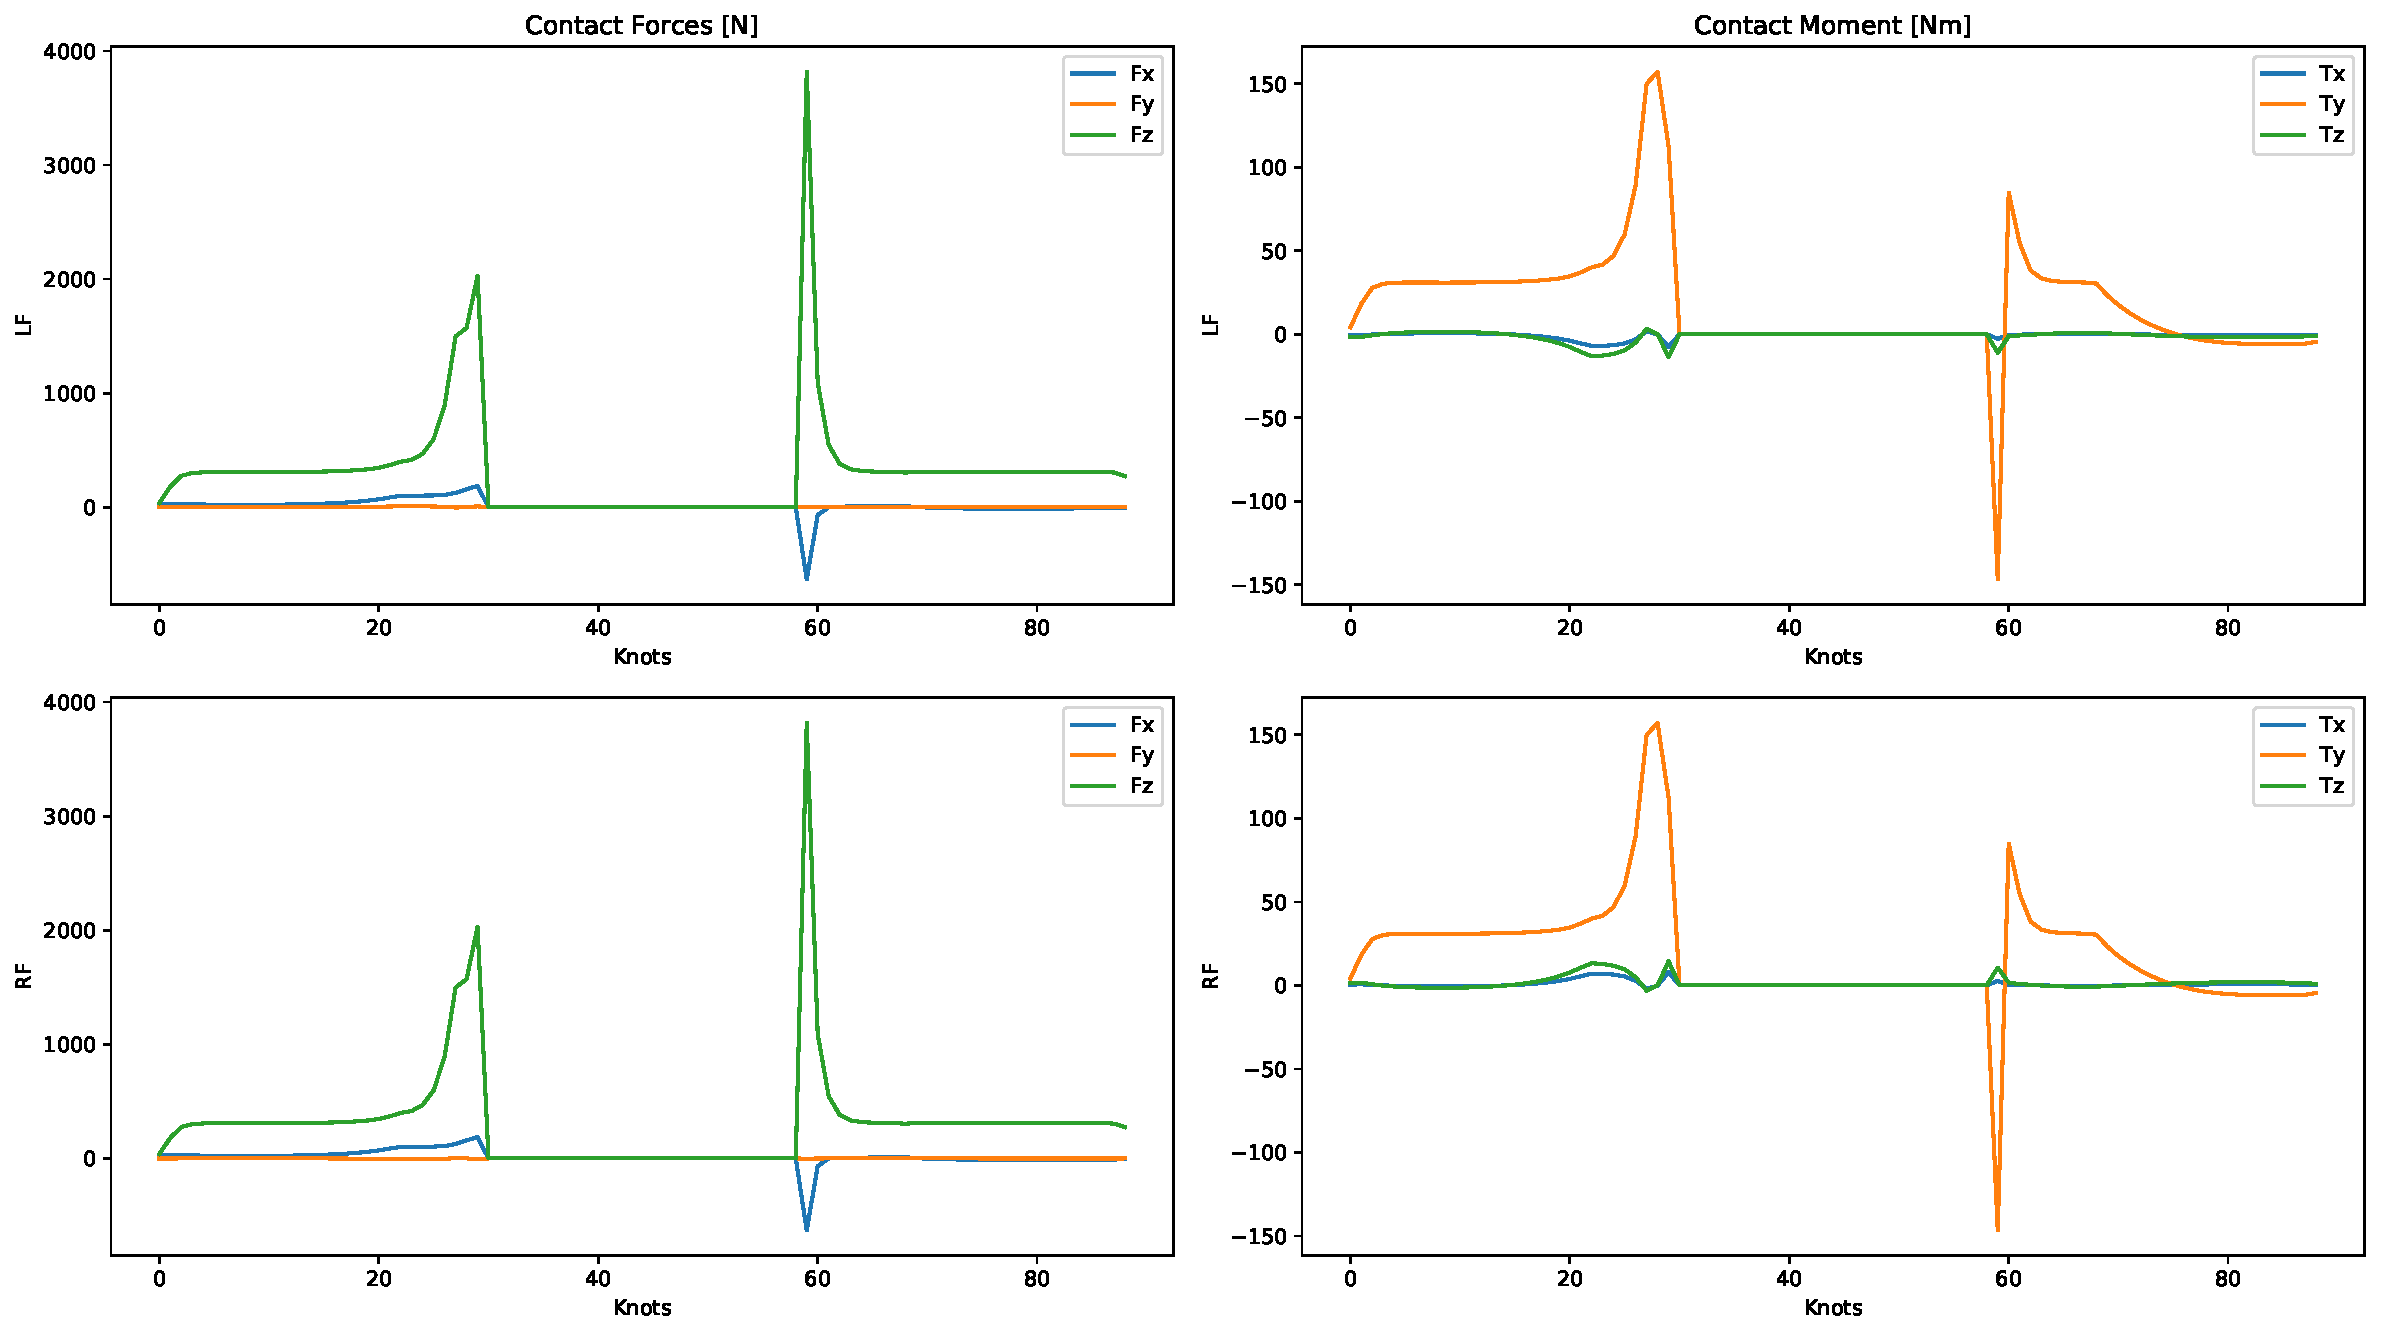
\includegraphics[width=1\textwidth]{fig/jumpForward/ContactWrenches}
\caption{Forward jump solution of the contact wrenches.}
\label{fig:jumpForward_ContactWrenches}
\end{figure} 

We have shown in \cref{sec:BipedEvaluation} that the proposed motion planning approach allows computation of dynamically balanced walking gaits. In the following, we want to investigate the feasibility of contact stability for highly-dynamic movements. \cref{fig:jumpForward_StabilityAnalysis} shows the stability analysis for the forward jumping task. It becomes clear that the \gls{CoP}s lie within the desired contact area of the left and right foot, respectively. Moreover, it can be observed that \gls{CoP}s are located more in the rear area of the sole of the foot before the jump or in the front area after landing. The first effect can be explained due to the angular momentum gained during descending of the base. The latter observation accounts for the rapid deceleration of the base motion in x-direction resulting from the instantaneous impact after the flight phase.    
\begin{figure}[h!]
\centering	
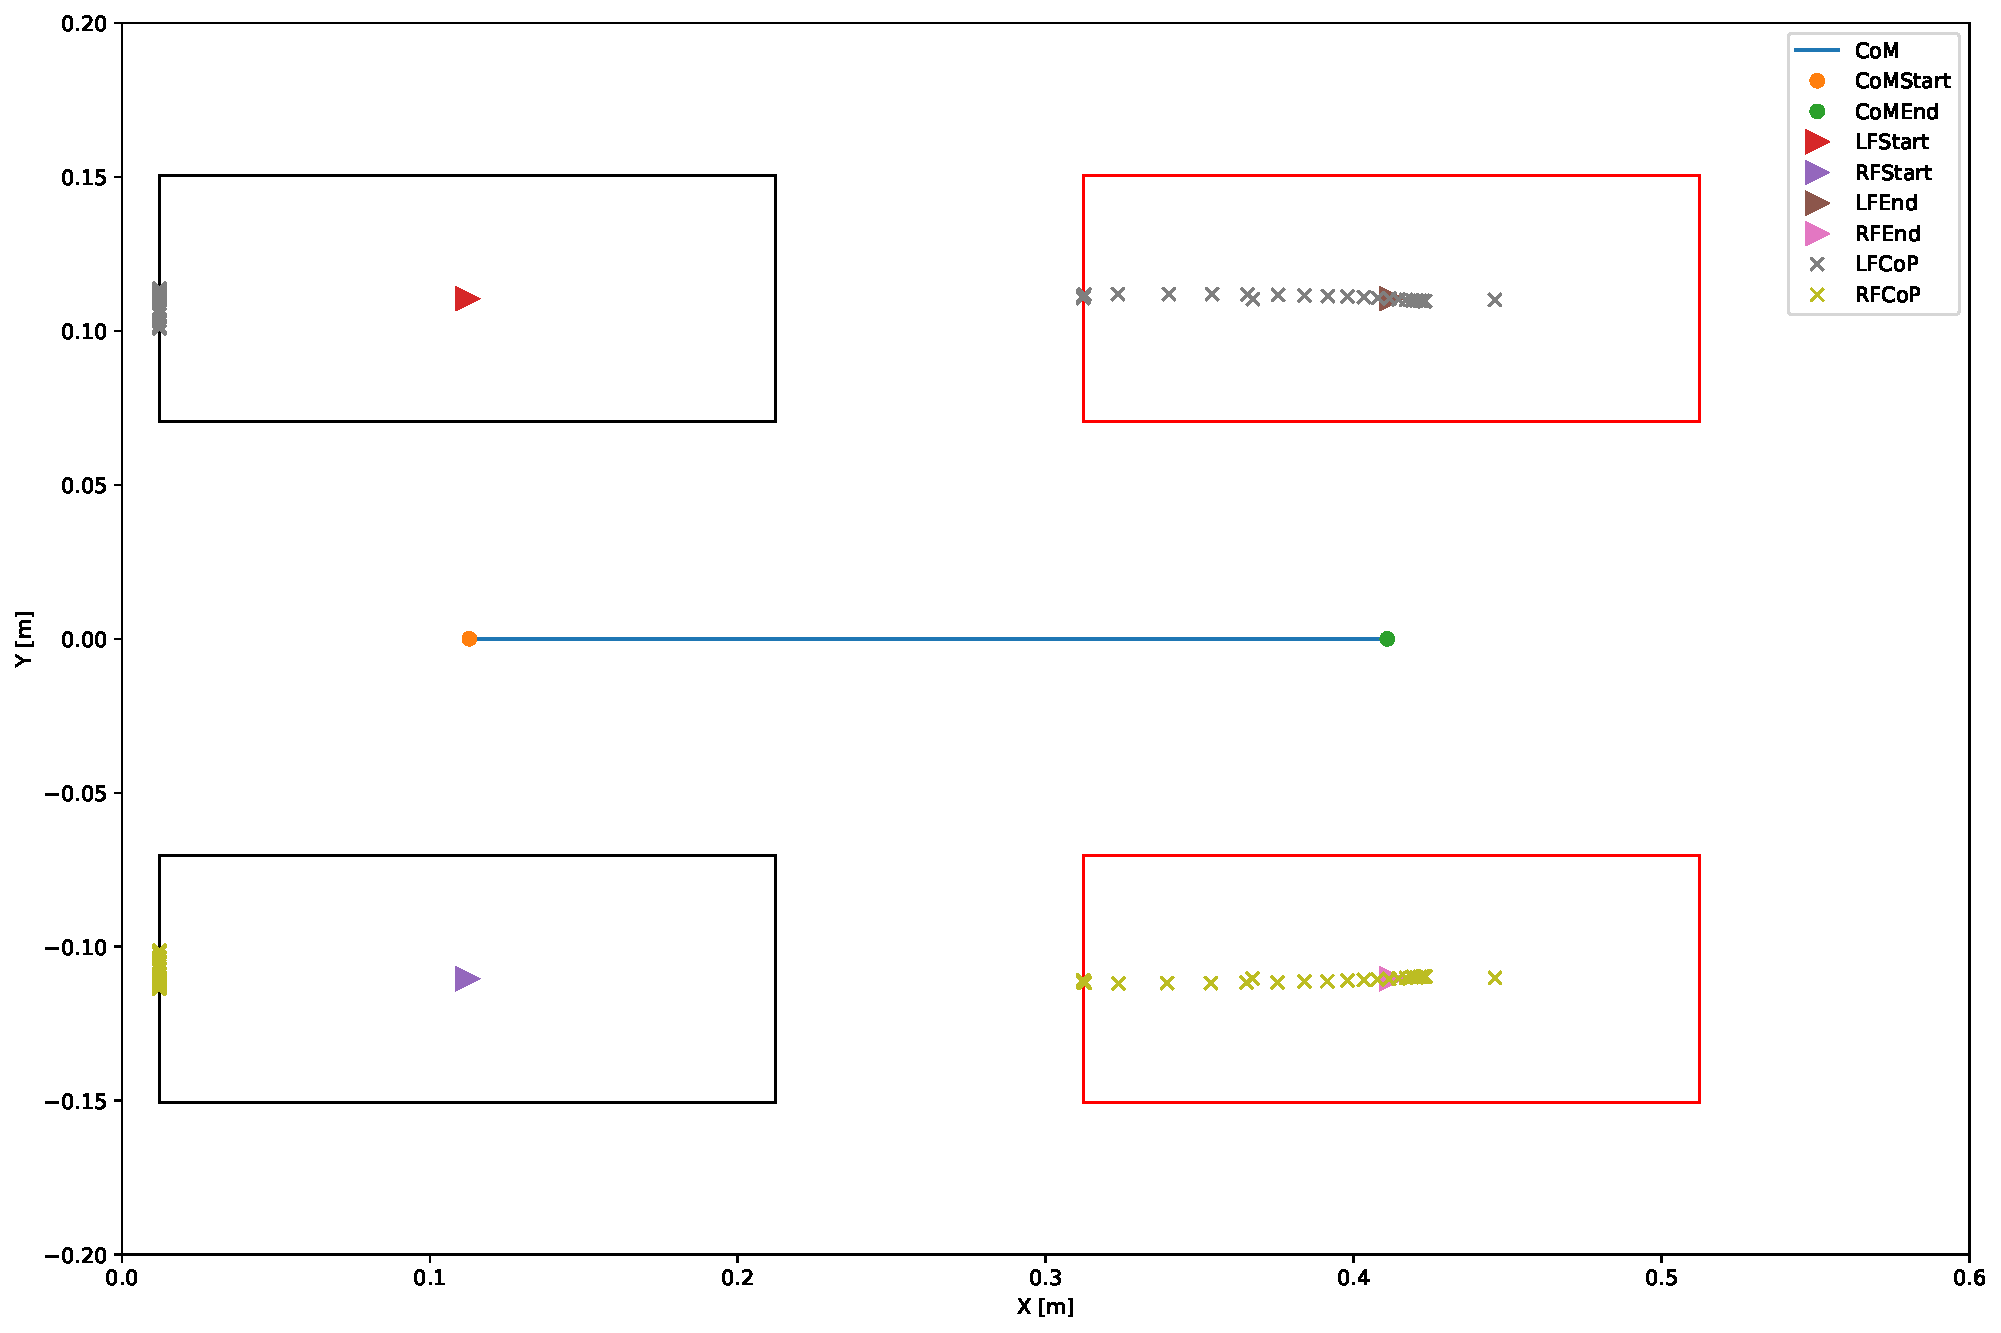
\includegraphics[width=.7\textwidth]{fig/jumpForward/StabilityAnalysis}
\caption{Stability analysis of the simple forward jump.}
\label{fig:jumpForward_StabilityAnalysis}
\end{figure} 

\subsection{Forward Jumping Over Multiple Obstacles}
Finally, we want to further increase the task dynamics and investigate the proposed motion planning approach for a challenging sequence of multiple forward jumps over obstacles. 

We build a sequence of \gls{OC} problems, as introduced in \cref{eqn:optimizationProblemSequence}, consisting of multiple forward jumps with increased jumping height and length (see \cref{tab:jumpObstacles}, accordingly. Since the RH5 humanoid was not designed for tasks of this dynamics, neither joint nor torque limits can be satisfied. In contrast to the simple vertical and forward jumps, this case study is supposed to proof the flexibility of the proposed motion planning approach rather than analyzing the system design. 

\begin{table}[t]
\centering
\caption{Multiple obstacles jumping characteristics and applied optimization constraints.}
\begin{tabular}{|ll|ll|}
\hline
\multicolumn{2}{|l|}{\textbf{Jump Characteristics}} & \multicolumn{2}{l|}{\textbf{Optimization Constraints}} \\ \hline
Number of jumps: & 3 	& Tasks: 			& Foot ($\Phi_1$) \\ \hline
Jump length:& 60 cm 	& Stability: 		& \gls{CoP} ($\Phi_3$), Friction Cone ($\Phi_4$)\\ \hline
Jump height:& 25 cm  	& Limits:   & / \\ \hline
Total time:& 1.2 s / jump  & Regularization: 	& Posture ($\Phi_7$), Torque ($\Phi_8$)\\ \hline
Step size:& 0.01 s & & \\ \hline
\end{tabular}
\label{tab:jumpObstacles}
\end{table}

\begin{figure}[h!]
\centering
\begin{subfigure}{.33\textwidth}
	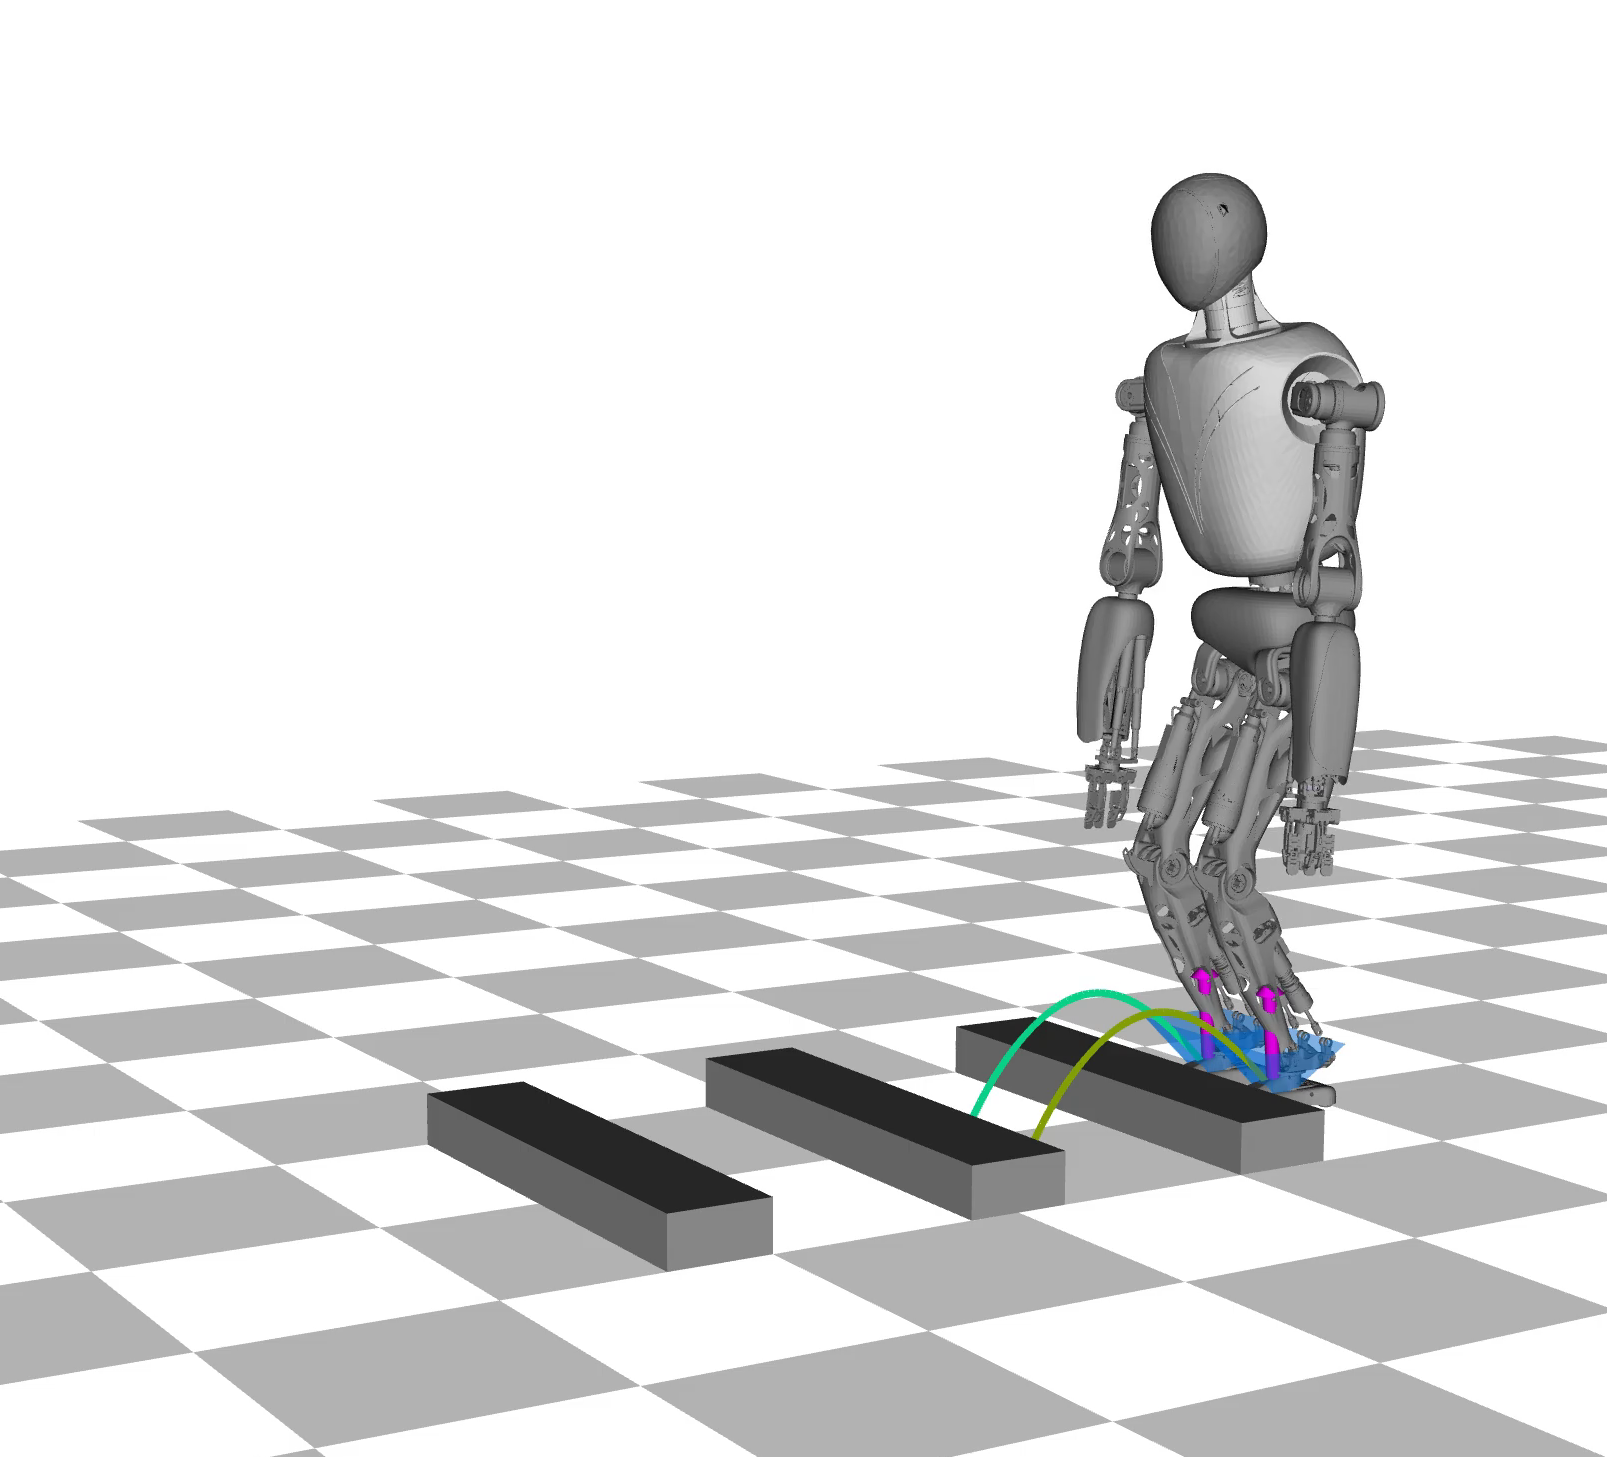
\includegraphics[width=1\linewidth]{fig/jumpObstacles/snaps/1x}
	\end{subfigure}%
\begin{subfigure}{.33\textwidth}
	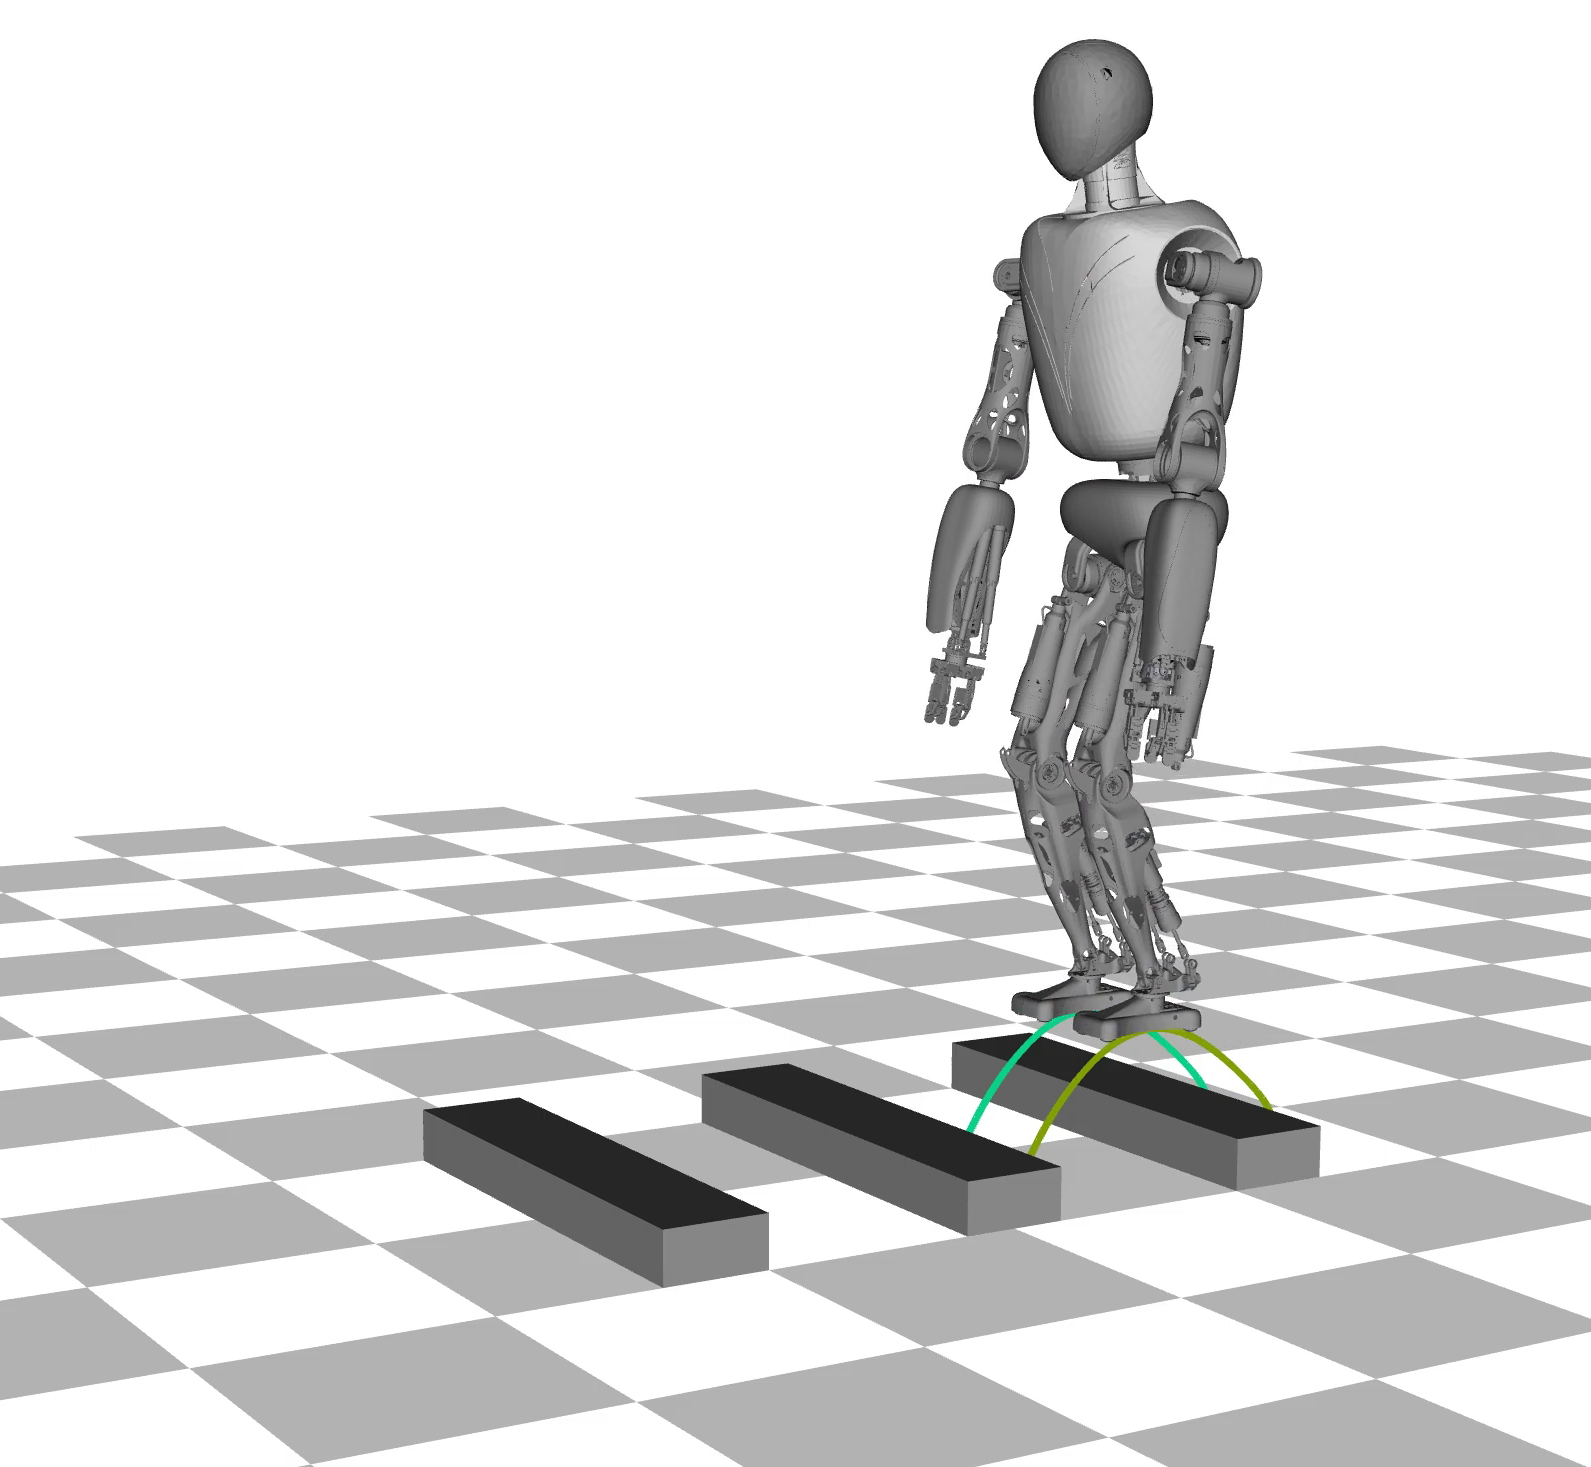
\includegraphics[width=1\linewidth]{fig/jumpObstacles/snaps/2x}
\end{subfigure}%
\begin{subfigure}{.33\textwidth}
	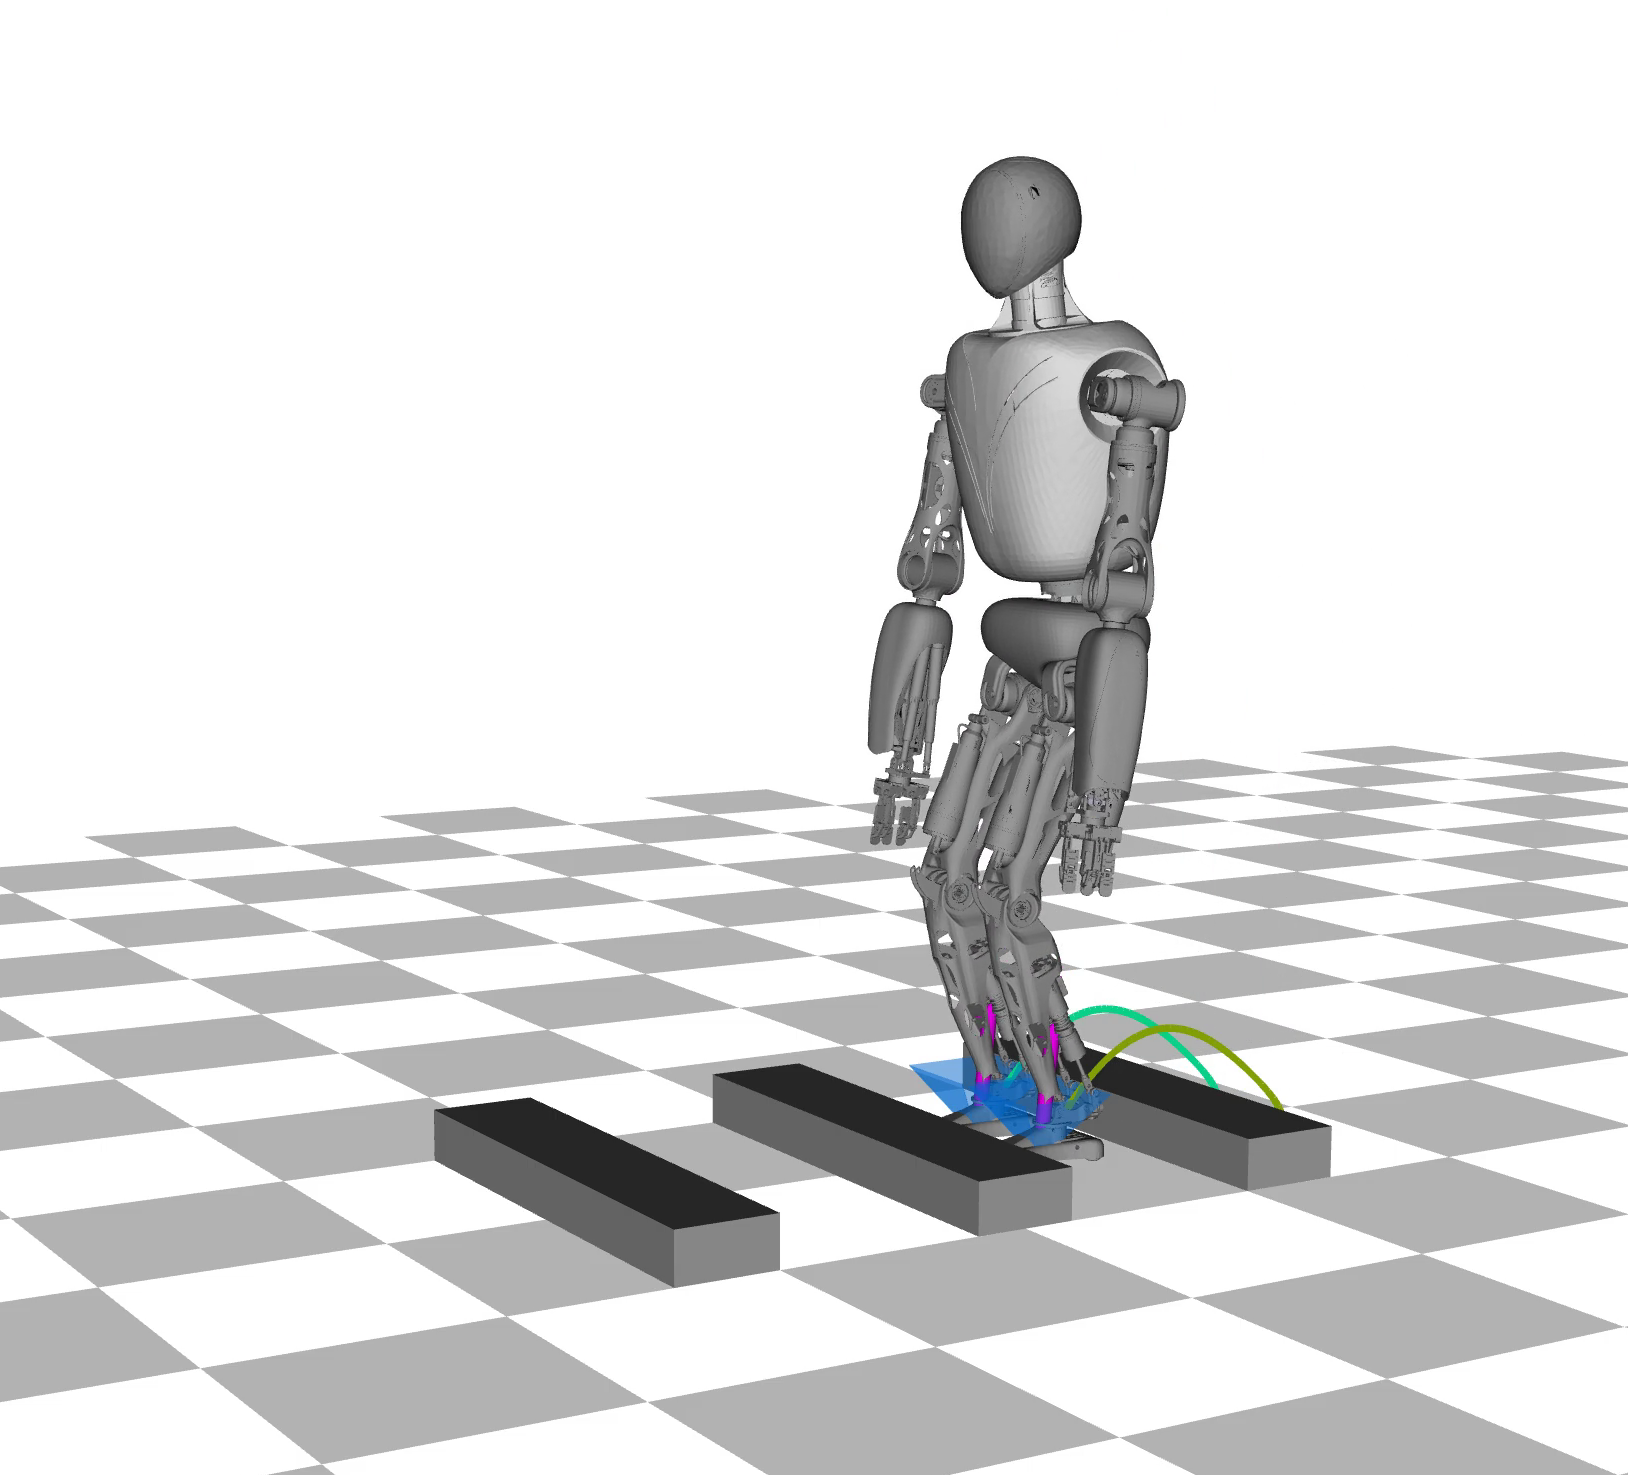
\includegraphics[width=1\linewidth]{fig/jumpObstacles/snaps/3x}
\end{subfigure}%
	
\begin{subfigure}{.33\textwidth}
	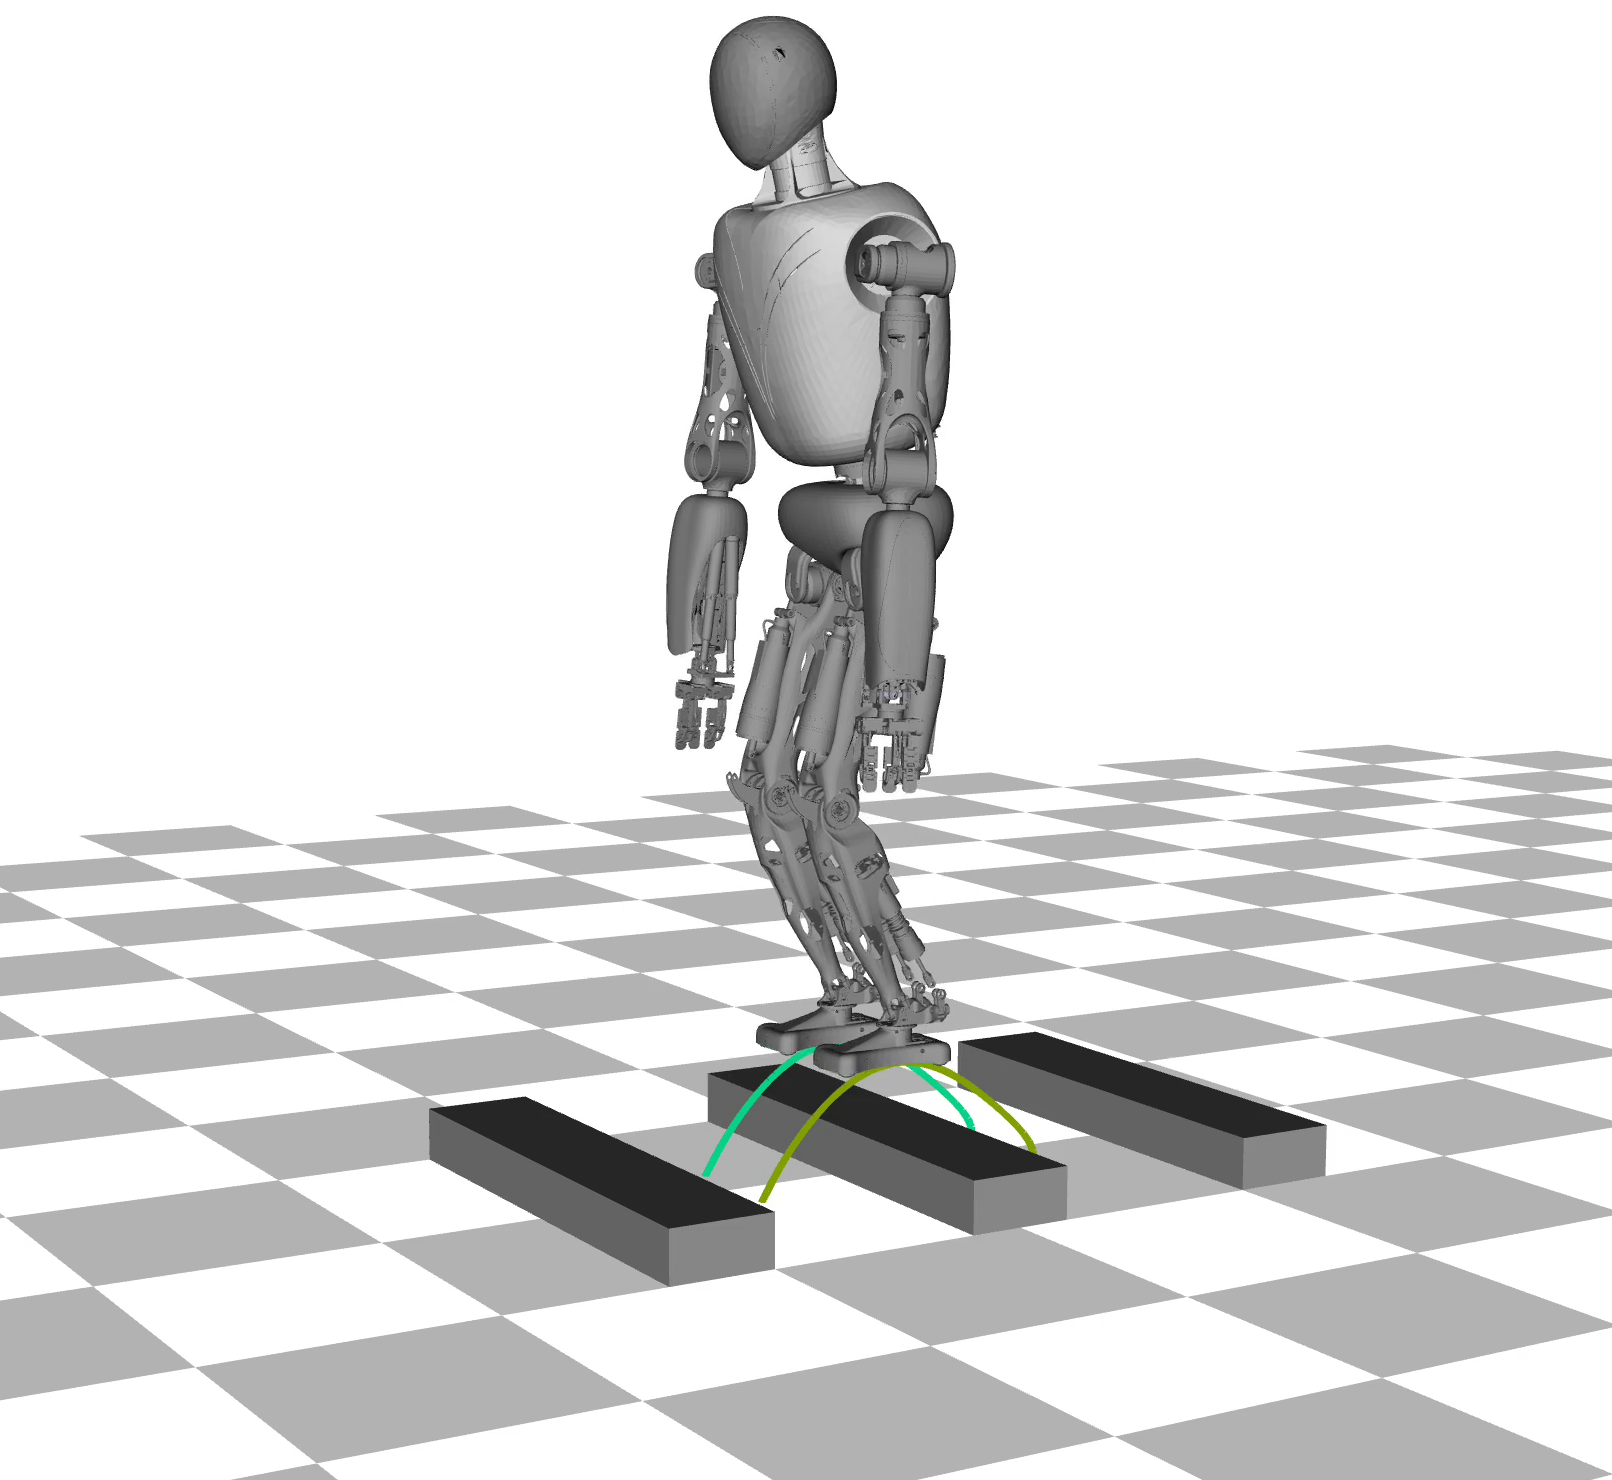
\includegraphics[width=1\linewidth]{fig/jumpObstacles/snaps/4x}
	\end{subfigure}%
\begin{subfigure}{.33\textwidth}
	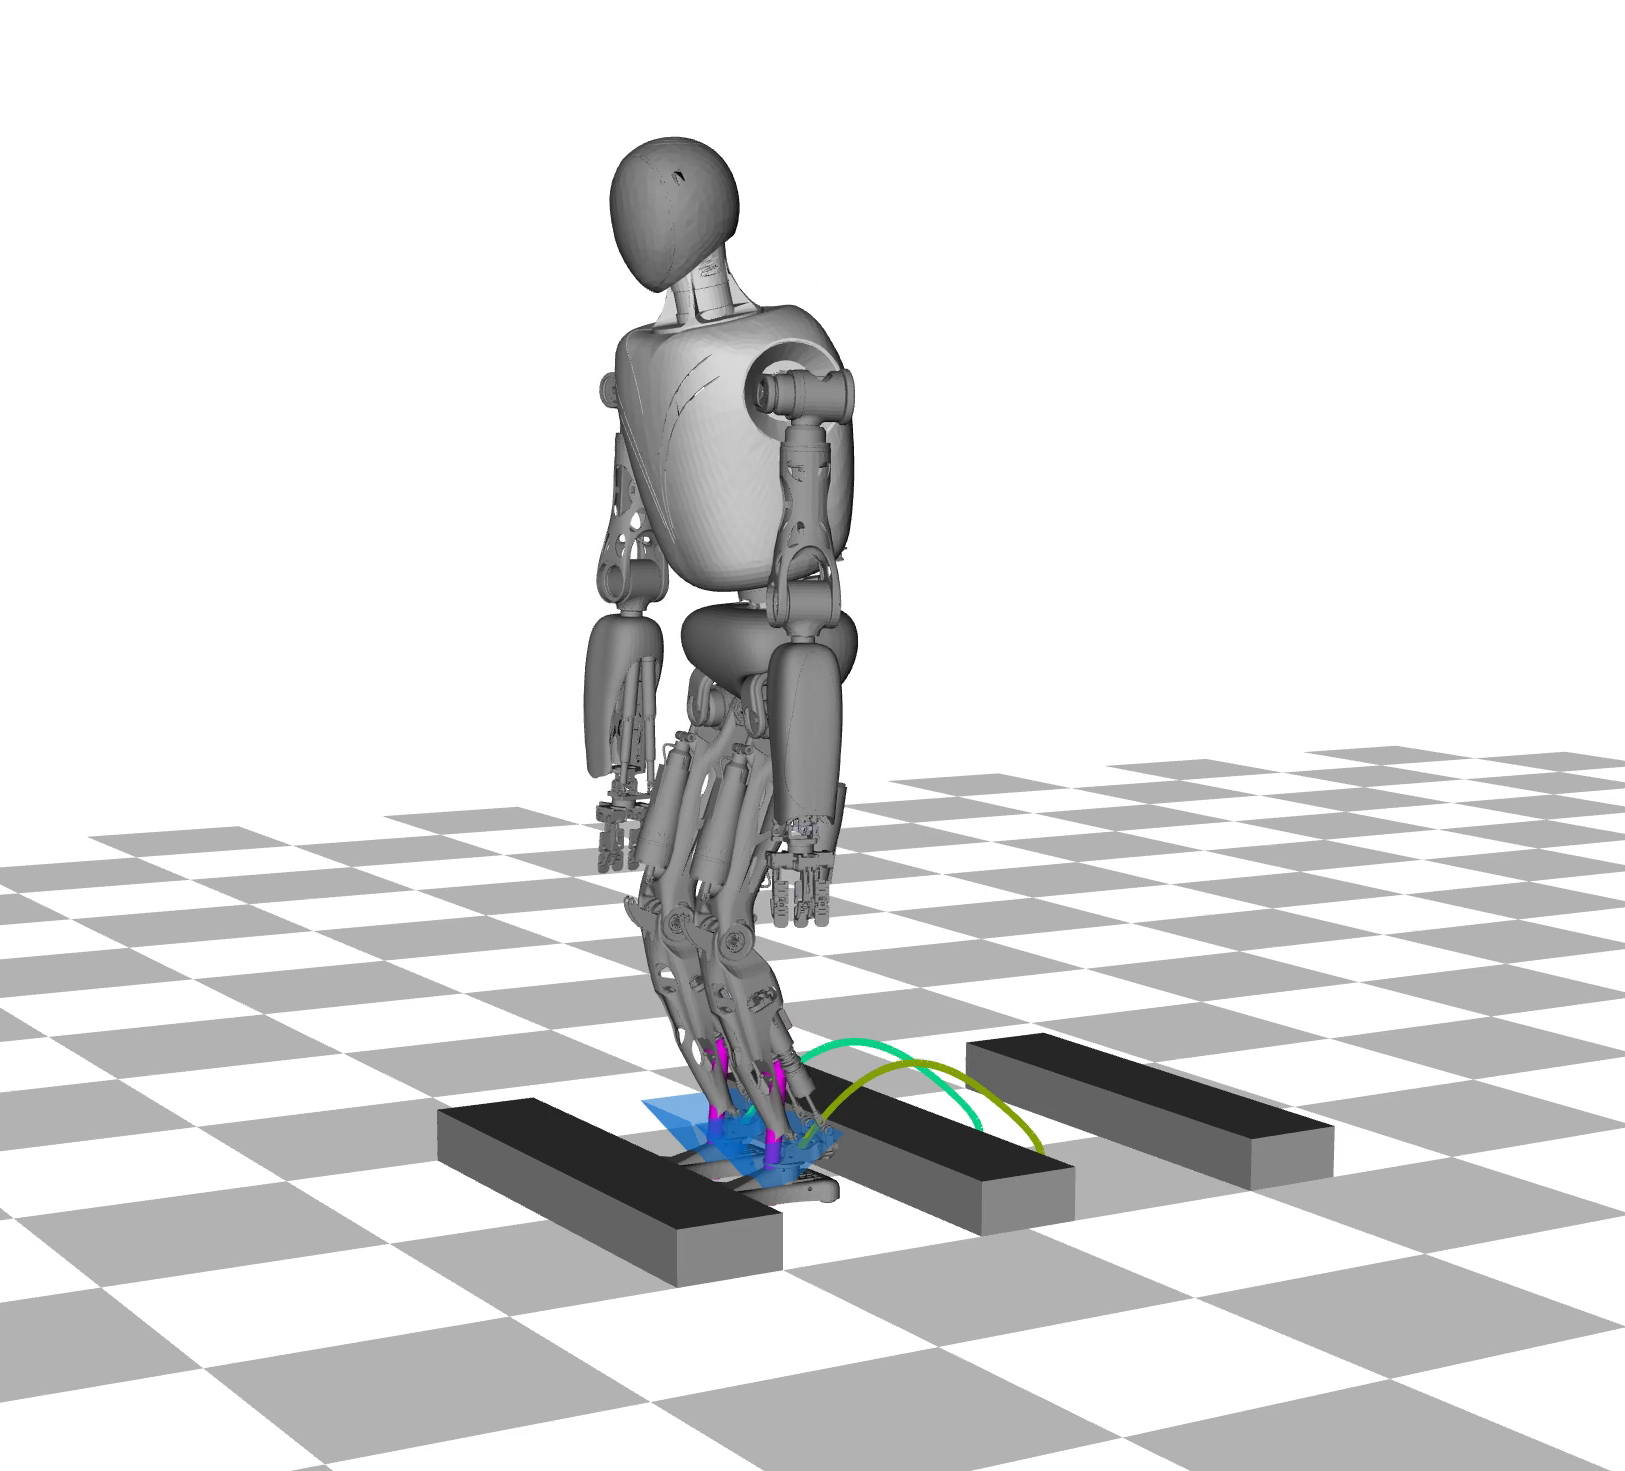
\includegraphics[width=1\linewidth]{fig/jumpObstacles/snaps/5x}
\end{subfigure}%
\begin{subfigure}{.33\textwidth}
	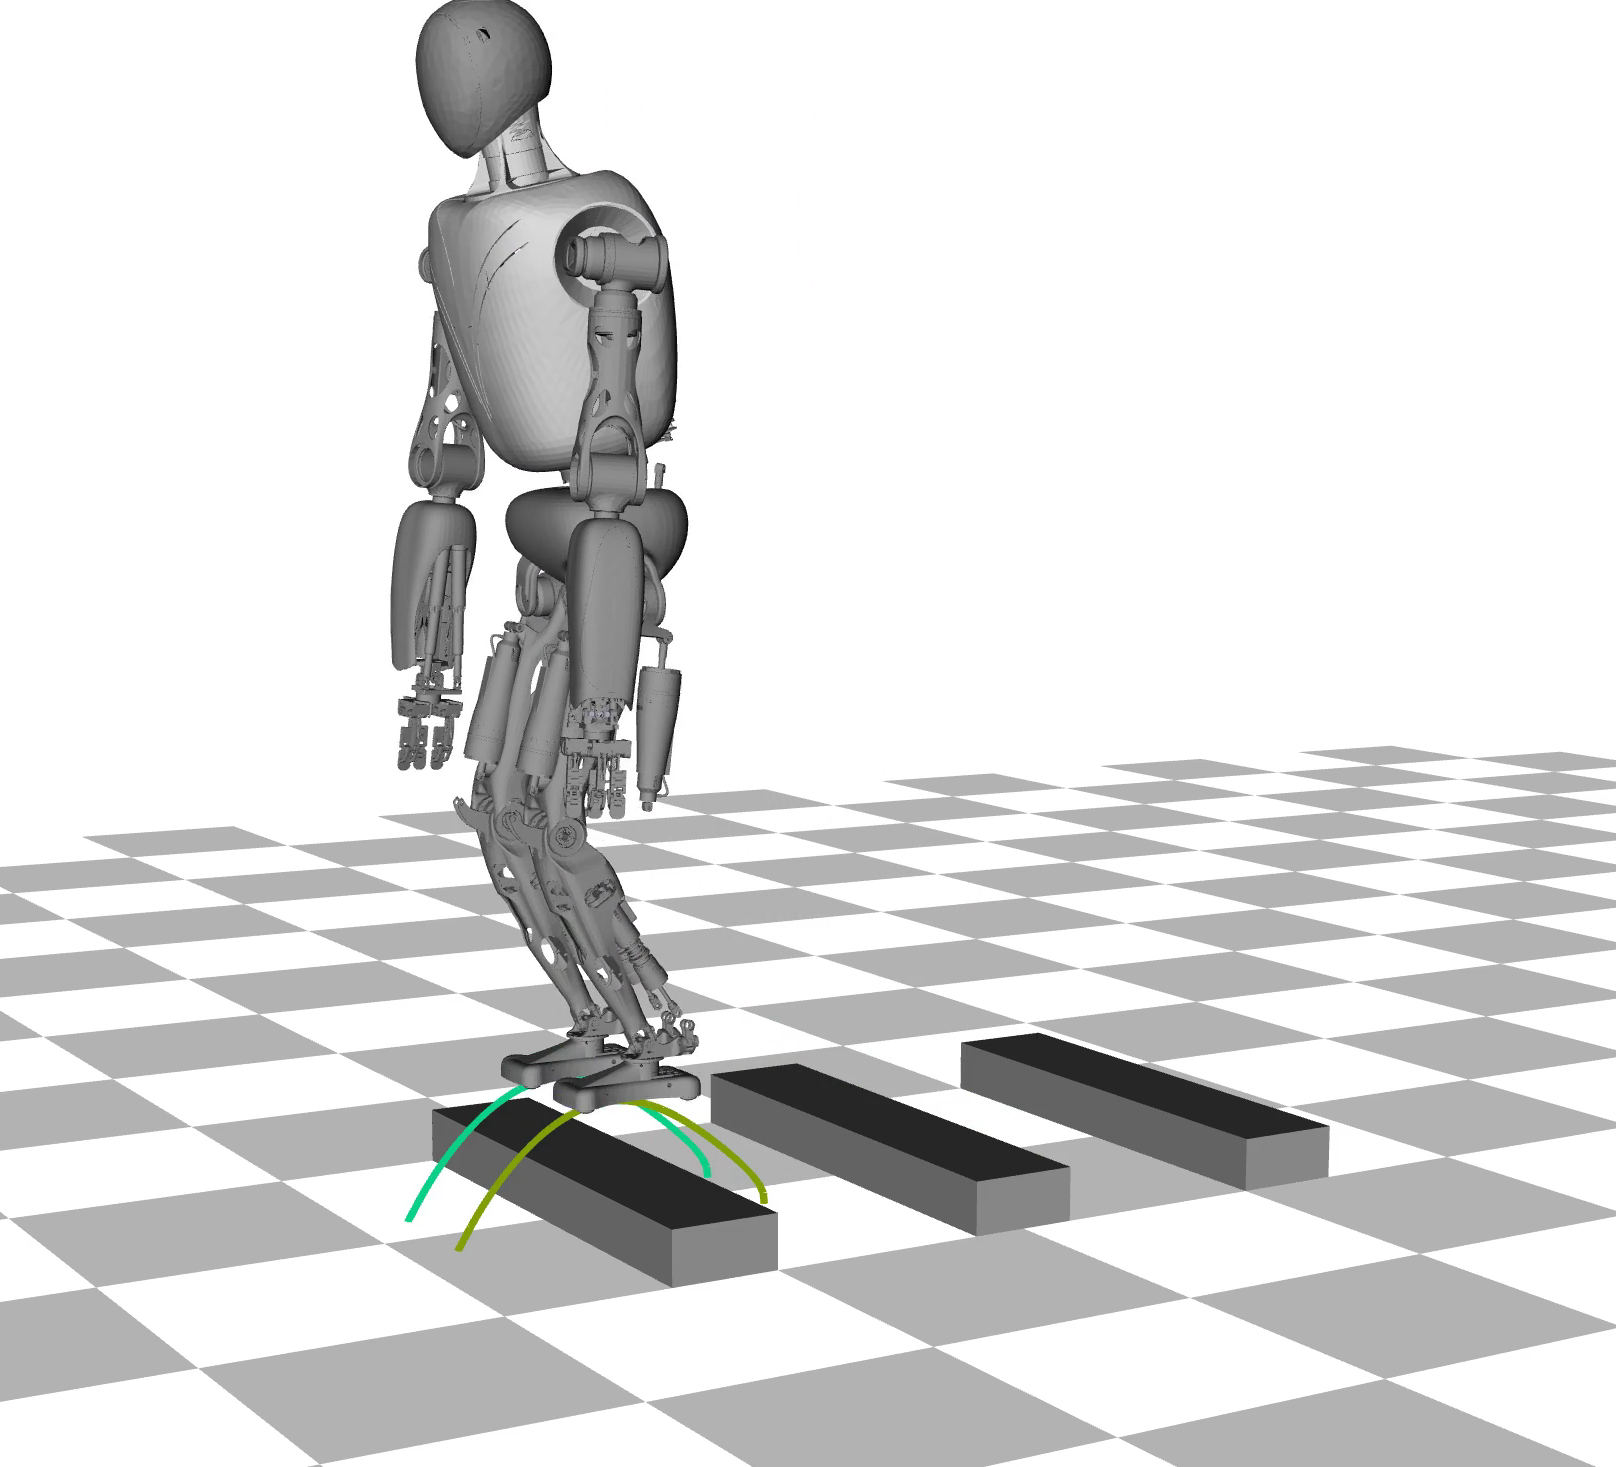
\includegraphics[width=1\linewidth]{fig/jumpObstacles/snaps/6x}
\end{subfigure}%

\begin{subfigure}{.33\textwidth}
	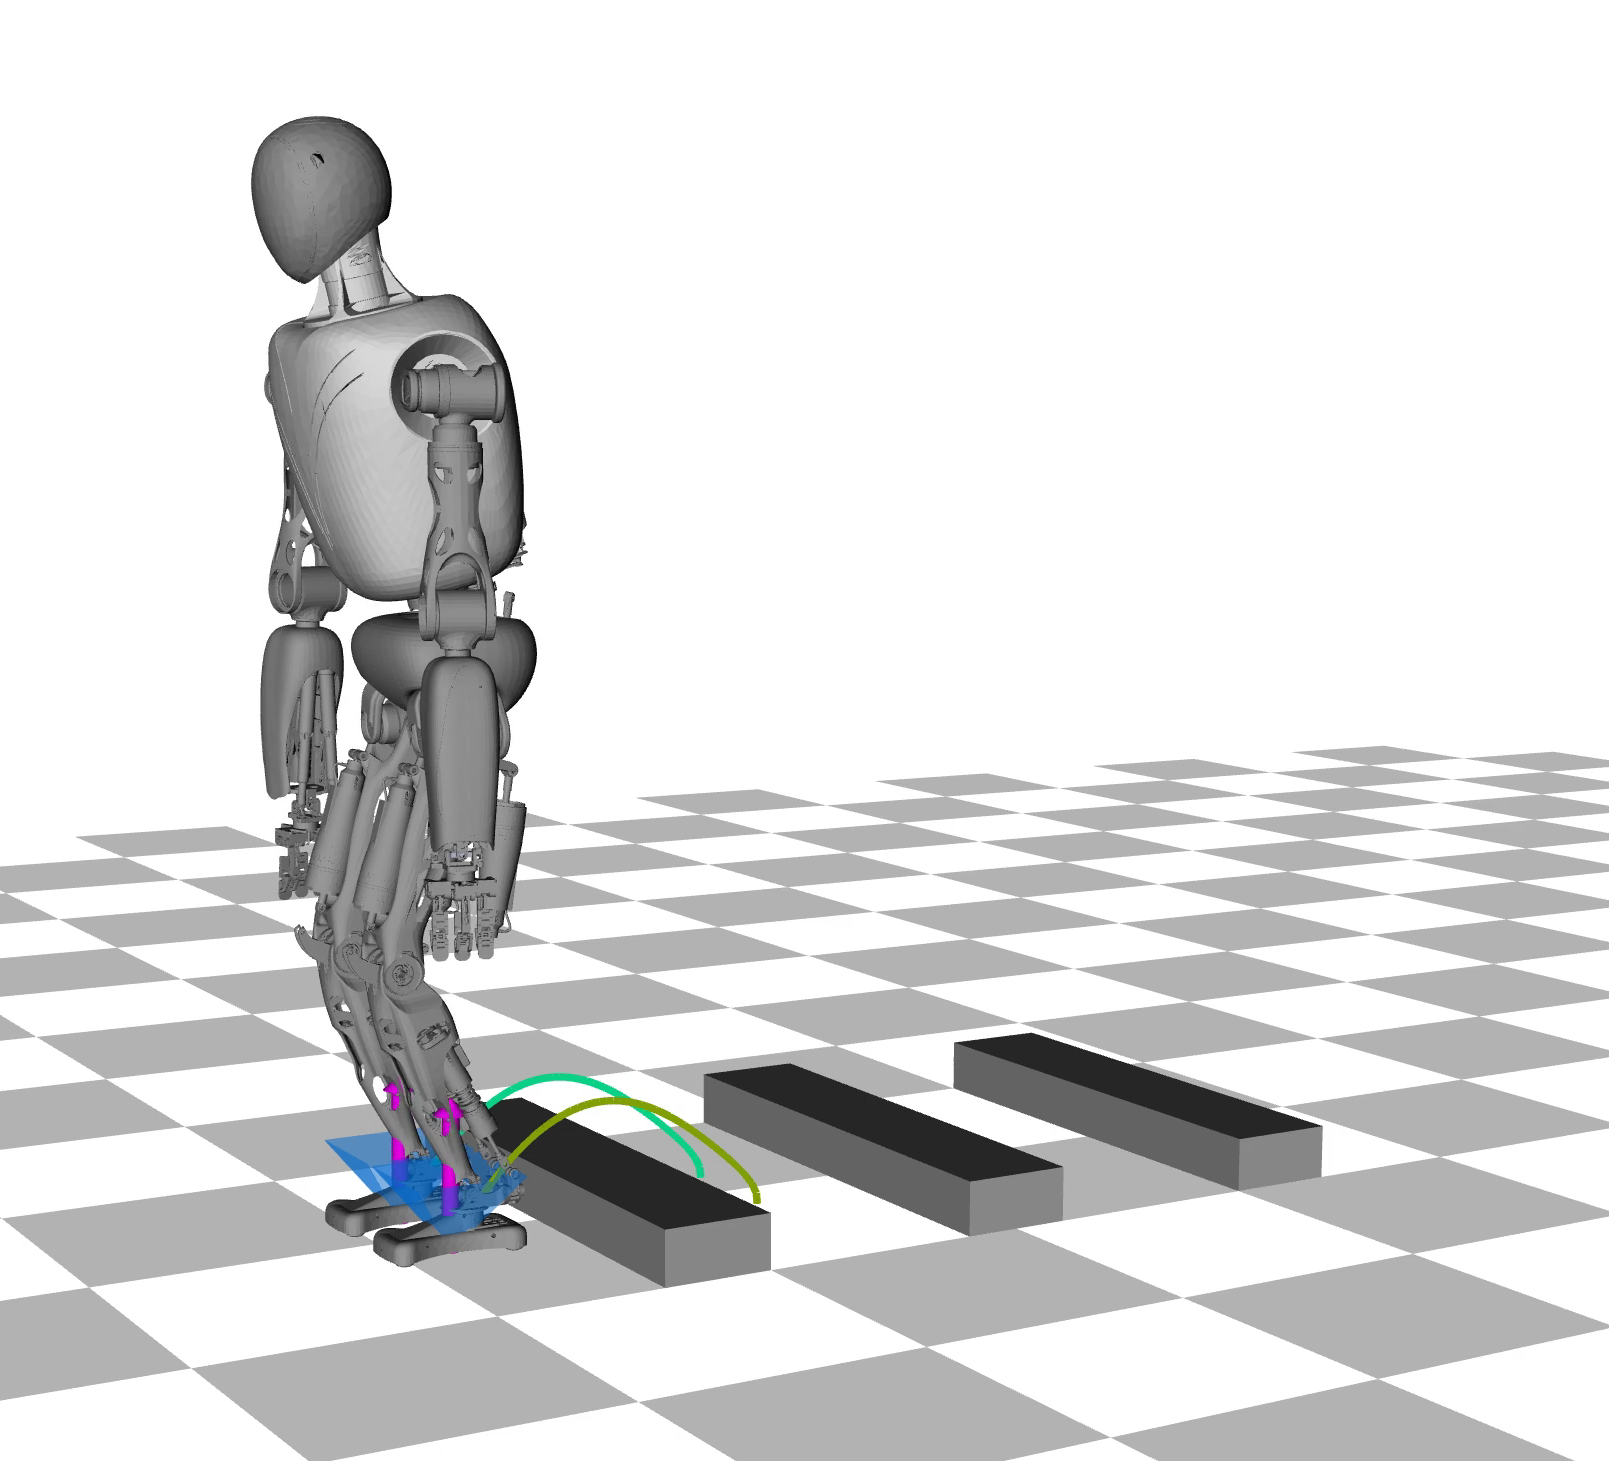
\includegraphics[width=1\linewidth]{fig/jumpObstacles/snaps/7x}
\end{subfigure}%

\caption{Multi-phase \gls{OC} problem of forward jumping over obstacles. Image order: column-wise, from top to bottom and left to right.}
\label{fig:jumpObstacles_Snaps}
\end{figure} 

Previously, we have demonstrated that the contact stability constrained \gls{DDP} allows computation of a simple forward jump with dynamical balanced motions. Following up, we want to study if the concept also holds for multiple forward jumps. 

\cref{fig:jumpObstacles_StabilityAnalysis} shows the obtained results for stability analysis for sequentially solving the sequence of optimization problems. The robot starts in an initial pose in \gls{DS}, performs a jump and recovers to the initial pose again. This \gls{OC} problem is repeated for three times with identical constraints and timings until the robot reaches the final \gls{DS} pose marked by red rectangles. As becomes evident, the contact stability constrained \gls{DDP} forces the \gls{CoP}s of both feet to lie within the desired contact area proofing for dynamically balanced motions. 

\begin{figure}[h!]
\centering	
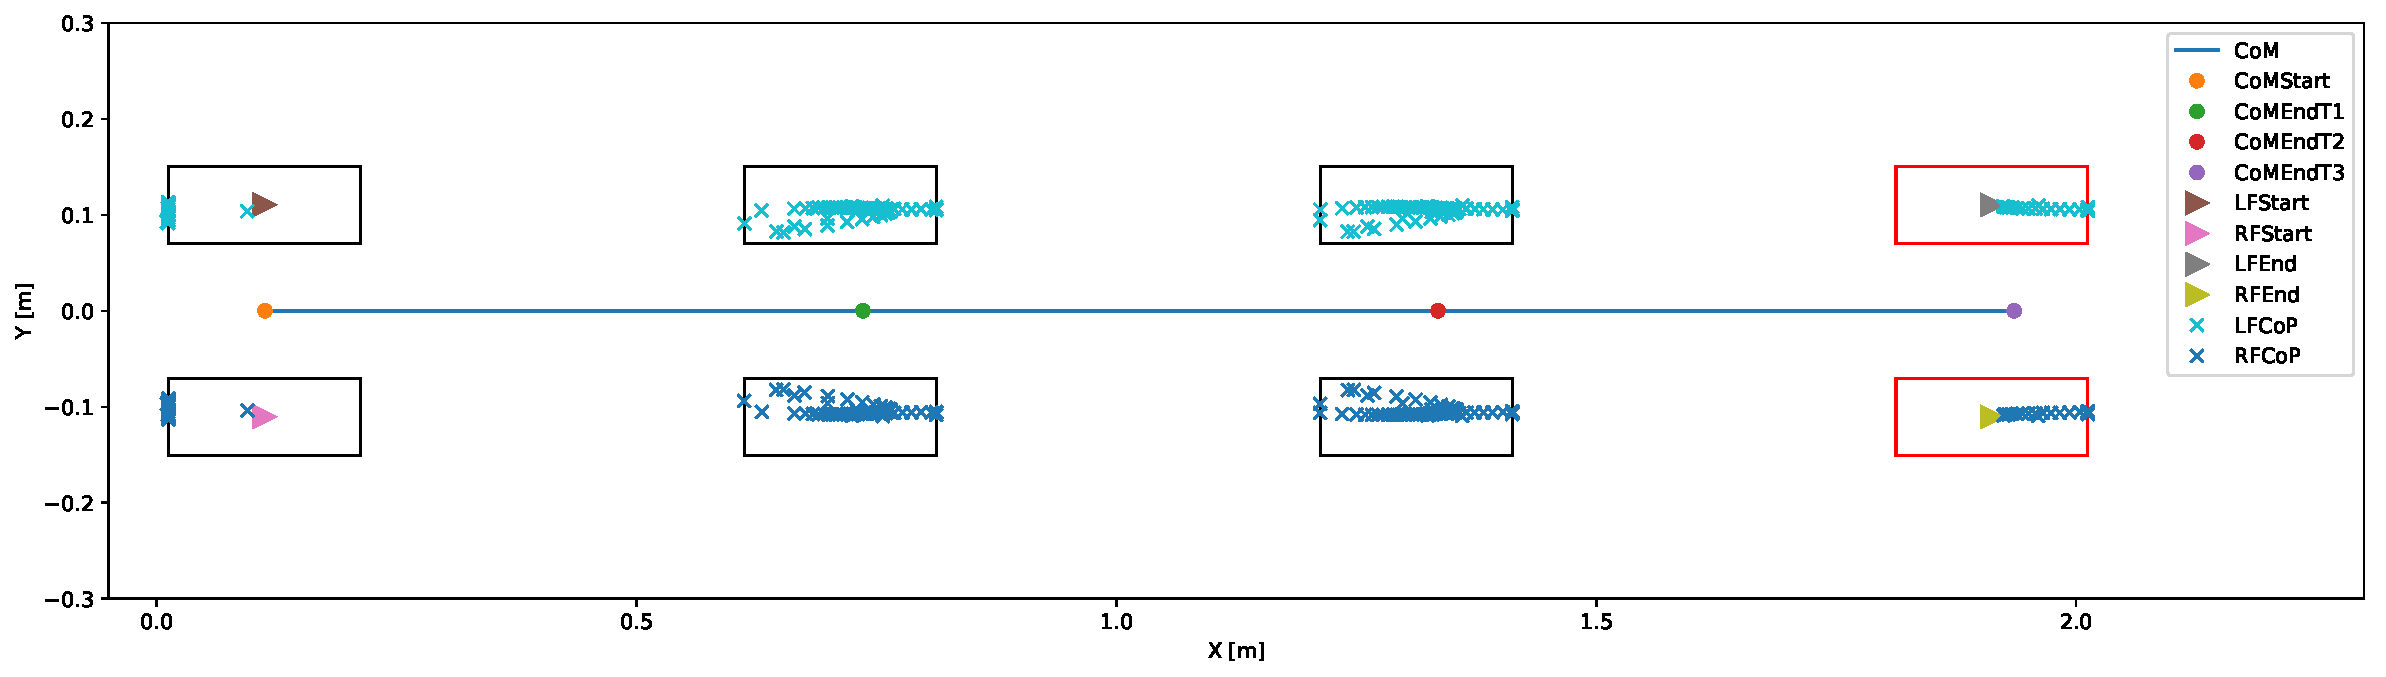
\includegraphics[width=1\textwidth]{fig/jumpObstacles/StabilityAnalysis}
\caption{Stability analysis of forward jumping over multiple obstacle.}
\label{fig:jumpObstacles_StabilityAnalysis}
\end{figure}

Recapitulating the results for the simple forward jump, we identified that the \gls{CoP}s are located in the rear area of the foot sole during takeoff. We can draw similar conclusions for the first jump of the multi-phase \gls{OC} problem. However, the \gls{CoP}s for the second and third jump do not share this pattern. This effect can be attributed to the dynamic forces already acting on the robot while the second and second impact phase, respectively.


\section{Evaluation of the System Design}\label{sec:HighlyIdentification}

This section presents an exhaustive study of the system limits of the RH5 humanoid robot based on the case studies introduced in the last section. The motivation is to form a basis of decision-making for future design iterations that allow the robot to perform highly-dynamic movements in real-world experiments.

The evaluation of the system design is performed by iteratively increasing the task complexity. We conduct multiple simulations with different jumping lengths $l$ and heights $h$ for the presented vertical jump ($h=$ 1 cm - 30 cm), forward jump ($l=$ 10 cm - 50 cm, $h=$ 10 cm) and forward jumping task over multiple obstacles ($l=$ 60 cm, $h=$ 25 cm), respectively (see \cref{tab:systemLimits}). Of particular interest here are the system-relevant limits, namely the valid  joint position and velocity ranges as well as the according maximum  motor torques. 

A few notes on the used notation in \cref{tab:systemLimits}: Checkmarks and crosses indicate whether the according limits are satisfied or not with the given movement. Checkmarks in brackets mean that a maximum torque needs to be applied for a period longer than 50 ms, which can not necessarily be provided by the real actuators. Underscored numbers along with the crosses declare for how many joints the according limit is exceeded.

In the following the results of the study are presented in detail and design guidelines are derived based on the conducted experiments. 

\begin{table}[t]
\centering
\caption{Capabilities of the RH5 humanoid to perform various highly-dynamic jumps (length $l$, height $h$) respecting the hardware limits, namely available motor torque and valid joint position and velocity ranges.}
\begin{tabular}{lccc}
\hline
& Position Limits & Torque Limits & Velocity Limits\\ \hline
Vertical Jump ($l=$ 0 cm) & & & \\
\quad\quad $h=$ 1 cm 		& \greencheckmark  & \greencheckmark & \greencheckmark \\
\quad\quad $h=$ 5 cm 		& \greencheckmark  & \greencheckmark & \redxmark$_3$ \\
\quad\quad $h=$ 10 cm 		& \greencheckmark & (\greencheckmark) & \redxmark$_3$  \\
\quad\quad $h=$ 20 cm 		& \greencheckmark  & (\greencheckmark) & \redxmark$_5$ \\
\quad\quad $h=$ 30 cm 		& \greencheckmark  & (\greencheckmark) & \redxmark$_7$ \\ \hline
Forward Jump ($h=$ 10 cm)& & & \\
\quad\quad $l=$ 10 cm 		& \greencheckmark  & (\greencheckmark) & \redxmark$_7$ \\
\quad\quad $l=$ 20 cm 		& \greencheckmark  & (\greencheckmark) & \redxmark$_7$ \\
\quad\quad $l=$ 30 cm 		& \greencheckmark  & (\greencheckmark) & \redxmark$_7$ \\
\quad\quad $l=$ 40 cm 		& \greencheckmark  & (\greencheckmark) & \redxmark$_7$ \\
\quad\quad $l=$ 50 cm 		& \greencheckmark  & (\greencheckmark) & \redxmark$_7$ \\ \hline
Obstacle Jump ($h=$ 25 cm)& & & \\
\quad\quad $l=$ 60 cm 		& \greencheckmark  & \redxmark$_5$ & \redxmark$_7$ \\ \hline
\end{tabular}
\label{tab:systemLimits}
\end{table}

\subsection{Design Guidelines derived from Vertical Jumping}
The vertical jumping tasks already gives good insights in the dynamic capabilities of the humanoid robot RH5. From \cref{tab:systemLimits} we can see that the smallest jump with a height of 1 cm can be realized with the system. This is remarkable, since the current design of the humanoid is not indented for the purpose of highly-dynamic movements. 

For jumps with a height of 5 cm or above we can draw the conclusion that velocity limits are can not be satisfied anymore. In the first case, body pitch and knee velocities are exceeded, which is reasonable since these form the main part of the motion. For the highest jump on the other hand, additionally limits for the ankle pitch joints and the shoulder roll joints turn out to be not sufficient anymore. These violations can be explained by the higher impact forces and increased arm swinging activities, respectively. 

\subsection{Design Guidelines derived from Forward Jumping}
In comparison to the simple vertical jump, the forward jumping tasks involves higher dynamic forces acting on the base and hence require even faster motions. To this end, none of the forward jumping tasks turned out to be feasible with the currently implemented velocity limits. Interestingly, the ankle pitch velocity turned out to be sufficient, while the hip joint velocity limits were exceeded. This effect may be explained by the reduced impact forces in z-direction, but the increased angular momentum necessary to move the base forward. 

Furthermore, we can draw similar conclusions for the torque feasibility from the vertical, forward and multiple jumping over obstacles tasks. Although the maximum torque available with the currently embedded motors are high enough, they may not be feasible with the real actuators. For the body pitch, knee and ankle pitch joints, these maximal torques have to be applied for a period longer than 50 ms. To prevent long-term damage to the system, the corresponding actuators should be redesigned with an appropriate safety factor. 





































 



